\documentclass[11pt]{article}

\usepackage[a4paper,margin=20mm]{geometry}
\usepackage[T1]{fontenc}
\usepackage[utf8]{inputenc}
\usepackage{xcolor}
\usepackage{graphicx}
\usepackage{float}
\usepackage{enumitem}
\usepackage{needspace}
\usepackage{microtype}
\usepackage[numbers,sort&compress]{natbib}
\usepackage{bibentry}
\usepackage{xr}
\usepackage[hidelinks]{hyperref}
\usepackage[most]{tcolorbox}
\usepackage{pifont}
\usepackage{fancyhdr}

% Quiet running navigation; preserve the existing text block and footer.
\setlength{\headheight}{14pt}
\pagestyle{fancy}
\fancyhf{}
\fancyhead[L]{\footnotesize\color{origingrey}TACO-2026-55\enspace\textperiodcentered\enspace Response}
\fancyhead[R]{\footnotesize\color{origingrey}\nouppercase{\leftmark}}
\fancyfoot[C]{\thepage}
\renewcommand{\headrulewidth}{0pt}
\renewcommand{\sectionmark}[1]{\markboth{#1}{}}

\newtcolorbox{blockquote}{
    enhanced,
    breakable,
    colback=gray!10,
    frame hidden,
    boxrule=0pt,
    arc=0mm,
    borderline west={2.5pt}{0pt}{gray!60},
    left=8pt,
    right=8pt,
    top=4pt,
    bottom=4pt
}

\definecolor{origingrey}{RGB}{78,78,78}
\definecolor{reviewblue}{RGB}{0,82,155}
\definecolor{revisionred}{RGB}{190,0,0}

\newenvironment{reviewcomment}
  {\par\noindent\begin{blockquote}\color{reviewblue}}
  {\color{black}\end{blockquote}\medskip}

\long\def\graysentence#1{{\color{origingrey}#1}}
\long\def\redsentence#1{{\color{revisionred}#1}}
\newcommand{\excerptlabel}[1]{\par\Needspace{3\baselineskip}\addvspace{4pt}\noindent\textcolor{black}{\textbf{#1}}\par\nopagebreak[4]}
\newcommand{\revisionlocation}[1]{\par\Needspace{5\baselineskip}\noindent #1\par\nopagebreak[4]}

\newenvironment{manuscriptexcerpt}
  {\small\begin{list}{}{\setlength{\leftmargin}{\leftmargini}%
     \setlength{\rightmargin}{\leftmargin}%
     \setlength{\topsep}{2pt}\setlength{\partopsep}{0pt}%
     \setlength{\parsep}{0pt}\setlength{\itemsep}{0pt}}\item\relax}
  {\end{list}}

% Use the revised manuscript's citation keys and numbers, never response-local numbering.
% Compile the manuscript first whenever its bibliography changes.
\externaldocument{../TACO_2026_FlusArch/main}
% Formatting helpers used by the manuscript's ACM-generated .bbl entries.
\providecommand{\bibfield}[2]{#2}
\providecommand{\bibinfo}[2]{#2}
\providecommand{\showarticletitle}[1]{#1}
\providecommand{\shownote}[1]{#1}
\providecommand{\showURL}{\relax}
\providecommand{\showISBNx}[1]{\unskip}
\providecommand{\showISBNxiii}[1]{\unskip}
\providecommand{\showISSN}[1]{\unskip}
\providecommand{\showCODEN}[1]{\unskip}
\providecommand{\showLCCN}[1]{\unskip}
\providecommand{\showeprint}[2][]{arXiv:#2}
\newcommand{\papercite}[1]{\begingroup\NoHyper\citep{#1}\endNoHyper\endgroup}
\makeatletter
% ACM entries may end with \newblock, which consumes the space before \par.
\long\def\BR@c@bibitem#1 #2\par{{%
  \let\protect\@unexpandable@protect
  \expandafter\gdef\csname BR@r@#1\@extra@b@citeb\endcsname
    {#2}}}
\newcommand{\loadpaperreferences}{%
  \begingroup
  \renewcommand{\bibliography}[1]{\input{../TACO_2026_FlusArch/main.bbl}}%
  \nobibliography*%
  \global\BR@starfalse
  \endgroup}
\newcommand{\paperreference}[1]{%
  \item[\normalfont\papercite{#1}]%
  \begingroup
  \let\hyper@natanchorstart\@gobble
  \let\hyper@natanchorend\@empty
  \let\emph\textit
  \textit{\bibentry{#1}}\par
  \endgroup}
\makeatother
\newenvironment{excerptreferences}
  {\par\smallskip\begingroup\color{black}\footnotesize
   \Needspace{4\baselineskip}\noindent References cited in this excerpt:\par\nopagebreak[4]
   \begin{description}[leftmargin=2.8em,labelwidth=2.5em,labelsep=.3em,font=\normalfont,style=multiline,itemsep=2pt,topsep=3pt]
   \sloppy}
  {\end{description}\endgroup\smallskip}

\newcommand{\name}{FluxArch}
\newcommand{\amd}{EPYC 9654 $\times$2}
\newcommand{\intel}{Gold 6430 $\times$2}
\newcommand{\ft}{FT 64-core}
\newcommand{\ampare}{NVIDIA A100}
\newcommand{\hopper}{NVIDIA H100}

\newcommand{\redone  }{\textcolor[rgb]{0.722, 0.329, 0.314}{\ding{182}}}
\newcommand{\redtwo  }{\textcolor[rgb]{0.722, 0.329, 0.314}{\ding{183}}}
\newcommand{\redthree}{\textcolor[rgb]{0.722, 0.329, 0.314}{\ding{184}}}
\newcommand{\redfour }{\textcolor[rgb]{0.722, 0.329, 0.314}{\ding{185}}}
\newcommand{\redfive }{\textcolor[rgb]{0.722, 0.329, 0.314}{\ding{186}}}

\setcounter{secnumdepth}{2}
\setcounter{tocdepth}{2}
\setlist{nosep}
\setlist[enumerate]{itemsep=3pt,topsep=3pt,parsep=0pt,partopsep=0pt}
\setlength{\intextsep}{8pt plus 2pt minus 2pt}

% A compact title without empty author/date rows.
\makeatletter
\renewcommand{\@maketitle}{%
  \begin{center}
    {\LARGE \@title\par}
  \end{center}
  \vspace{8pt}}
\makeatother

\title{Response to the Editors and Reviewers\\
\large Manuscript TACO-2026-55}
\author{}
\date{}

\begin{document}
\loadpaperreferences
\maketitle

We sincerely thank the editors and the reviewers for their careful reading and constructive comments. We have revised the manuscript accordingly. For clarity, reviewer comments are reproduced in \textcolor{reviewblue}{blue}, our responses are in black, and the corresponding changes in the revised manuscript are shown in \textcolor{revisionred}{red}.

\tableofcontents
\clearpage

\section{Reviewer 1}

\subsection{Question 1}
\begin{reviewcomment}
Some aspects of the architecture lack a clear justification. FluxArch uses 8 compute tiles, each containing 8 clusters with 16 cores each, but the rationale behind this organization is not explained. Was this hierarchy derived from design-space exploration or empirical evaluation? How would a different hierarchy (For example, 16 -{}> 8 -{}> 8 instead of 8 -{}> 8 -{}> 16) perform?
\end{reviewcomment}

We sincerely thank you for your helpful and constructive suggestion.

\begin{enumerate}[label=(\arabic*)]
\setlength{\emergencystretch}{1em}
\item \textbf{Hierarchy sizing.} Our hierarchy is selected bottom-up through empirical evaluation. We added hierarchy-configuration sweeps under a common requirement that every workload retain at least 80\% scaling efficiency. The results select 16 cores per cluster and eight clusters per Compute Tile as the largest sharing domains satisfying this criterion across all five workloads, yielding a 128-core tile and a 1,024-core system.

\revisionlocation{The selected hierarchy and its link to the sizing study are summarized in \textbf{Section 4.1}.}

\excerptlabel{Original (Section 4.1, page 9):}\par
\begin{manuscriptexcerpt}
\graysentence{Sixteen \name\ Cores form a \name\ Cluster, which shares a cache and TLB.} \graysentence{Eight \name\ Clusters form a \name\ Tile, which is equipped with a multi-channel memory controller optimized for bandwidth-intensive MCPT applications like XSBench.} \graysentence{At the top level, the system comprises eight Compute Tiles and a centralized Switch Tile.} \graysentence{As shown in Table~1, we carefully balanced cache capacity against the large database requirements of MCPT to optimize area.} \graysentence{A key architectural departure in \name\ is the omission of a shared L3 cache.} \graysentence{Prior analysis indicates that expanding cluster-local L2 capacity offers superior performance-per-area and reduces coherence complexity compared to a monolithic L3.} \graysentence{This design aligns with throughput-oriented architectures that prioritize L2 proximity for massive TLP, making \name\ more GPU-like while retaining independent control flows.}
\end{manuscriptexcerpt}
\excerptlabel{Revised (Section 4.1, page 8):}\par
\begin{manuscriptexcerpt}
\redsentence{We size the hierarchy bottom-up using an empirical criterion that every evaluated workload must retain at least 80\% scaling efficiency.} \redsentence{The sweeps in Section~6.6 select 16 cores per cluster and 8 clusters per Compute Tile, yielding a 128-core tile.} \redsentence{Eight such tiles are interconnected through a centralized Switch Tile to form a 1,024-core system.}
\end{manuscriptexcerpt}
\item \textbf{Alternative hierarchy configurations.} We also added direct evaluations of the $16\times8\times8$ organization, together with $32\times4\times8$ and $32\times8\times4$, while holding the total core count at 1,024, the memory system at 32 channels, and every crossbar (XBar) at no more than 64 endpoints. The revised evaluation shows geometric-mean performance of 1.00, 0.96, 0.93, and 0.89 for these four organizations, respectively. The selected $8\times8\times16$ organization performs best overall because fewer cluster-bound MPI processes preserve communication locality for CORAL2-P1, CORAL2-P2, CTS2 and Homogeneous, while the alternatives benefit XSBench through greater aggregate cluster-local level-2 (L2) cache capacity and bandwidth.
\revisionlocation{The design-space constraints, bottom-up sweeps, and alternative-hierarchy trade-offs are explained in \textbf{Section 6.6}.}

\excerptlabel{Added (Section 6.6, pages 19--20):}\par
\begin{manuscriptexcerpt}
\redsentence{We first constrain the design space in three ways.} \redsentence{We cap each XBar at 64 endpoints to avoid impractical arbitration, wiring, and timing complexity.} \redsentence{We fix both the system scale at 1,024 cores and the memory system at 32 channels, so alternative hierarchies have identical compute and off-chip bandwidth resources.} \redsentence{Within this space, we require every workload to retain at least 80\% scaling efficiency and size the sharing domains from the bottom up.} \redsentence{Fig.~17(a) varies the number of cores per cluster: 16 cores retain 81.46\%--97.98\% efficiency, whereas at 32 cores four workloads fall below the criterion.} \redsentence{Fig.~17(b) then fixes 16-core clusters and varies the number of clusters per tile: eight clusters retain 81.02\%--94.93\%, whereas at 16 clusters only CTS2 remains above 80\%.} \redsentence{These sweeps establish 16 cores per cluster and eight clusters per tile as the largest per-level configurations that satisfy the criterion across all workloads, while smaller configurations remain viable alternatives.}

\redsentence{We next compare $8\times8\times16$ against three representative alternatives that also satisfy these constraints: $16\times8\times8$, $32\times4\times8$, and $32\times8\times4$, which progressively distribute the same 1,024 cores across more, smaller sharing domains.} \redsentence{Fig.~17(c) reports geometric-mean normalized performance of 1.00, 0.96, 0.93, and 0.89 for these four configurations, respectively.} \redsentence{The per-workload results reveal two opposing effects.} \redsentence{For CORAL2-P1, CORAL2-P2, CTS2 and Homogeneous, performance declines as the number of cluster-bound MPI processes rises from 64 to 128, 128, and 256.} \redsentence{More process boundaries increase communication overhead, which is material because particle exchange already accounts for 16.93\%--31.80\% of cycle-tracking time in Table~6(c).} \redsentence{XSBench has no inter-process particle exchange and instead benefits from the higher aggregate capacity and bandwidth of 128, 128, and 256 cluster-local L2s.} \redsentence{This sensitivity agrees with Table~6(a), where XSBench has the largest database, lowest L2 read hit rate, and highest normalized DRAM read traffic.} \redsentence{Thus, $8\times8\times16$ best balances communication locality and aggregate L2 resources across the workload suite.}
\end{manuscriptexcerpt}
\par\noindent\begin{minipage}{\linewidth}
\revisionlocation{The per-level scaling sweeps and normalized alternative-hierarchy results are added in \textbf{Figure~17(a--c)}.}

\excerptlabel{Added (Figure~17, page 19):}\par
% Revised manuscript: Figure 17
\begin{figure}[H]
  \centering
  \fbox{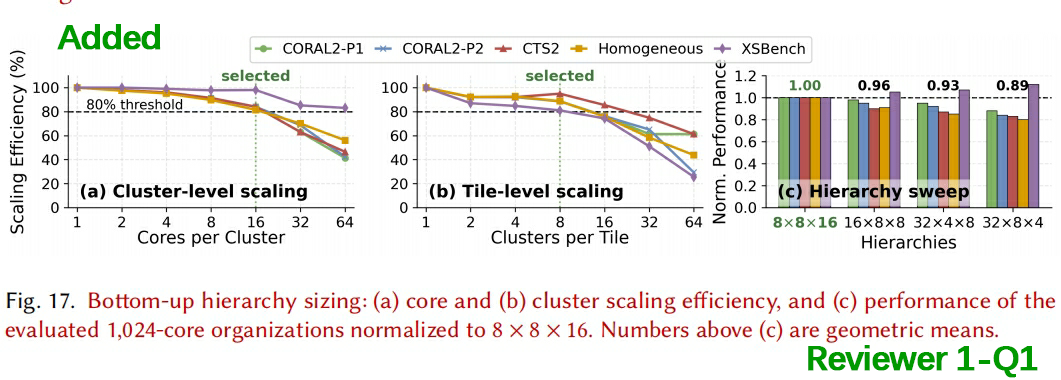
\includegraphics[width=0.9\textwidth]{news/R1-Q1-fig17.png}}
\end{figure}
\end{minipage}\par\medskip

\par\noindent\begin{minipage}{\linewidth}
\revisionlocation{The database sizes, L2 hit rates, and DRAM traffic supporting the XSBench explanation are reported in \textbf{Table~6(a)}.}

\excerptlabel{Added (Table~6(a), page 18):}\par
% Revised manuscript: table 6(a)
\begin{figure}[H]
  \centering
  \fbox{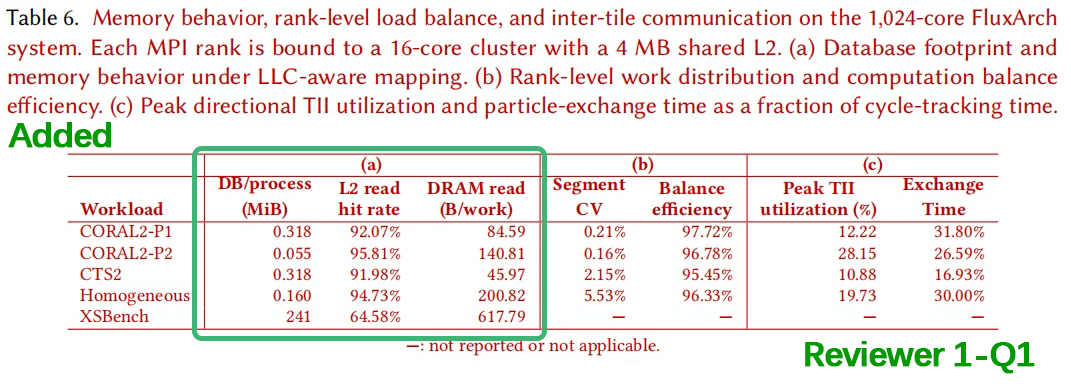
\includegraphics[width=0.9\textwidth]{news/R1-Q1-tab6a.png}}
\end{figure}
\end{minipage}\par\medskip

\end{enumerate}


\subsection{Question 2}
\begin{reviewcomment}
The thread affinity and spatial decomposition strategies described in Section 5 may introduce load imbalance, causing some cores to handle significantly more work than others. The authors acknowledge this as a limitation and suggest dynamic partitioning as a future work direction, but it would still be valuable to at least quantify the resulting imbalance and its impact on performance.
\end{reviewcomment}

Our static affinity and spatial decomposition assign one MPI rank to each cluster, so stochastic particle histories can create unequal work across the 64 ranks. We added a rank-level evaluation using both completed segments and accumulated tracking-kernel time rather than assuming perfect balance. The coefficient of variation (CV) of kernel time is only 1.17\%--2.01\%, balance efficiency is 95.45\%--97.72\%, and the resulting computation-side tail loss is at most 4.55\% for the evaluated inputs. These results indicate that static affinity and spatial decomposition maintain balanced computation across clusters for the evaluated workloads at 1,024 cores, with limited computation-side loss from load imbalance.

\revisionlocation{The rank-level load-balance method and its computation-side impact are evaluated in \textbf{Section 6.5}.}

\excerptlabel{Added (Section 6.5, pages 18--19):}\par
\begin{manuscriptexcerpt}
\redsentence{\textbf{Load Balance.}} \redsentence{Table~6(b) quantifies the concern that static affinity and spatial decomposition may assign unequal work to clusters.} \redsentence{We record completed segments and accumulated tracking-kernel time separately for all 64 ranks.} \redsentence{Segment-count CV ranges from 0.16\% to 5.53\%; because stochastic segments can follow different paths and incur different costs, count variation does not translate proportionally into execution-time variation.} \redsentence{Kernel-time CV remains 1.17\%--2.01\%.} \redsentence{We define balance efficiency as the mean rank-level kernel time divided by the maximum rank-level kernel time, since the slowest rank determines the computation tail.} \redsentence{The resulting efficiency is 95.45\%--97.72\%, corresponding to an estimated computation-side tail loss of at most 4.55\%.} \redsentence{These results indicate that static affinity and spatial decomposition maintain balanced computation across clusters for the evaluated workloads at 1,024 cores, with limited computation-side loss from load imbalance.}
\end{manuscriptexcerpt}
\par\noindent\begin{minipage}{\linewidth}
\revisionlocation{The segment-count variation and balance efficiency are added in \textbf{Table~6(b)}.}

\excerptlabel{Added (Table~6(b), page 18):}\par
% Revised manuscript: Table 6(b)
\begin{figure}[H]
  \centering
  \fbox{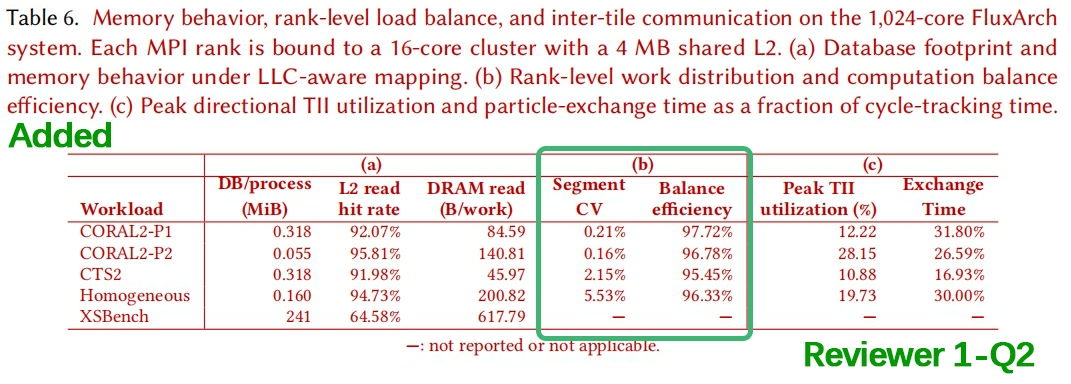
\includegraphics[width=0.9\textwidth]{news/R1-Q2-tab6b.png}}
\end{figure}
\end{minipage}\par\medskip

\subsection{Question 3}
\begin{reviewcomment}
A missing aspect of the experimental setup is the modeling of inter-tile communication. More details are needed to ensure reproducibility and properly contextualize the results.
\end{reviewcomment}

Inter-tile communication is explicitly modeled rather than treated as zero-cost functional transfer. We expanded the evaluation methodology to specify that MPI messages traverse the guest network stack, Intel Gigabit Ethernet (IGbE) endpoints, and \texttt{DistEtherLink}-based Tile Interconnection Interfaces (TIIs) and therefore incur protocol processing, packetization, serialization, and modeled link latency. We also added per-TII traffic and end-to-end particle-exchange measurements: the busiest direction reaches 10.88\%--28.15\% of the 1-Gb/s link capacity, while traffic CV across the eight TIIs is 0.50\%--2.42\%. Thus, communication has a measurable execution cost, but TII saturation or traffic imbalance is not the bottleneck in these experiments.

\revisionlocation{The MPI transport path and communication-cost measurement method are specified in \textbf{Section 6.1}.}

\excerptlabel{Added (Section 6.1, page 13):}\par
\begin{manuscriptexcerpt}
\redsentence{\textbf{Inter-Tile Communication Modeling.}} \redsentence{The eight Compute Tiles are connected to the Switch Tile through eight bidirectional Tile Interconnection Interfaces (TIIs).} \redsentence{In distributed full-system gem5, each TII is modeled using a \texttt{DistEtherLink} and an IGbE endpoint, with the directional 1-Gb/s capacity in Table~1 and the modeled inter-tile latency.} \redsentence{MPI messages traverse the guest network stack and these modeled links and are therefore subject to software protocol processing, packetization, link serialization, and inter-tile latency rather than zero-cost functional communication.} \redsentence{We use the Ethernet-device counters to measure transmitted bytes and directional utilization at every TII.} \redsentence{Quicksilver's cycle-tracking timers separately measure end-to-end particle-exchange time, including buffer handling, MPI communication and waiting, and receive-side particle management.}
\end{manuscriptexcerpt}
\revisionlocation{The measured TII utilization and traffic balance are analyzed in \textbf{Section 6.7}.}

\excerptlabel{Added (Section 6.7, page 21):}\par
\begin{manuscriptexcerpt}
\redsentence{Table~6(c) reports peak directional TII utilization and the particle-exchange share of cycle-tracking time.} \redsentence{Across CORAL2-P1, CORAL2-P2, CTS2 and Homogeneous, \name\ injects 1.37--1.46 bytes of inter-tile traffic per completed segment.} \redsentence{The busiest directional TII reaches only 10.88\%--28.15\% of its modeled 1-Gb/s capacity.} \redsentence{Bidirectional link traffic is also well balanced: its coefficient of variation across the eight TIIs is 0.50\%--2.42\%.} \redsentence{Thus, the communication-driven spatial mapping avoids TII hotspots, and the evaluated links remain below saturation.}
\end{manuscriptexcerpt}
\par\noindent\begin{minipage}{\linewidth}
\revisionlocation{The peak directional TII utilization and particle-exchange share are reported in \textbf{Table~6(c)}.}

\excerptlabel{Added (Table~6(c), page 18):}\par
% Revised manuscript: Table 6(c)
\begin{figure}[H]
  \centering
  \fbox{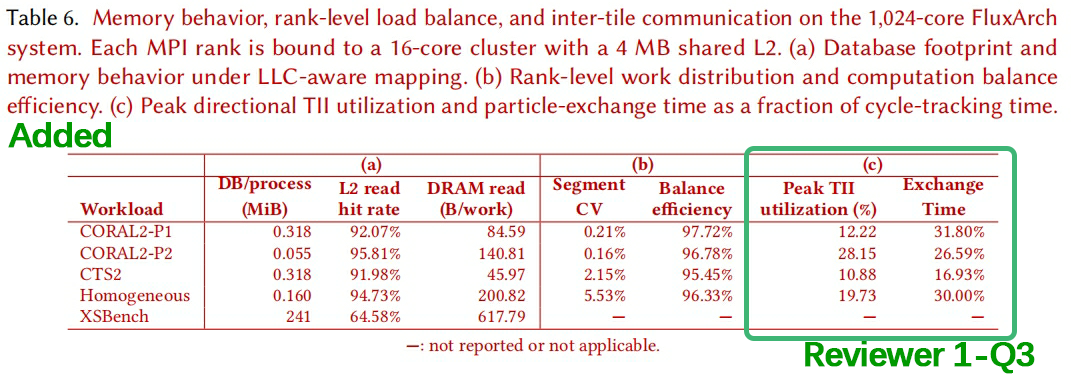
\includegraphics[width=0.9\textwidth]{news/R1-Q3-tab6c.png}}
\end{figure}
\end{minipage}\par\medskip


\subsection{Question 4}
\begin{reviewcomment}
In the experimental setup, there is no mention of random seed control or variability between runs, which are important details as MCPT is stochastic.
\end{reviewcomment}

We use the same fixed workload-default pseudorandom seed for each workload across platforms to support reproducibility. Each experiment is repeated 10 times under exclusive-platform and stable-thermal conditions, and we report the arithmetic mean of the workload-native performance metric. Across the platform--workload configurations in Figure~13(a), the throughput coefficient of variation (CV) ranges from 0.1\% to 6.2\%, and from 0.1\% to 0.4\% for \name. These values quantify run-to-run variability with the seed held fixed. We have added the repetition count and CV ranges to \textbf{Section 6.1}.

\revisionlocation{The seed policy and reporting of run-to-run variability are clarified in \textbf{Section 6.1}.}

\excerptlabel{Added (Section 6.1, page 14):}\par
\begin{manuscriptexcerpt}
\redsentence{\textbf{Reproducibility and Run-to-Run Variability}.} \redsentence{All platforms use fixed workload-default pseudorandom seeds (Table~\ref{tab:benchmarks}).} \redsentence{Each experiment is repeated 10 times, and we report the arithmetic mean of the workload-native performance metric.} \redsentence{Runs use exclusive platforms under stable thermal conditions.} \redsentence{For Fig.~13(a), the throughput coefficient of variation (CV) is 0.1\%--6.2\% across platform--workload configurations and 0.1\%--0.4\% for \name.}
\end{manuscriptexcerpt}

\par\noindent\begin{minipage}{\linewidth}
\revisionlocation{The workload seeds are specified in \textbf{Table~4}, which corresponds to \textbf{Table~2} in the original manuscript.}

\excerptlabel{Original (Table~2, page 14):}\par
% Original manuscript: Table 2
\begin{figure}[H]
  \centering
  \fbox{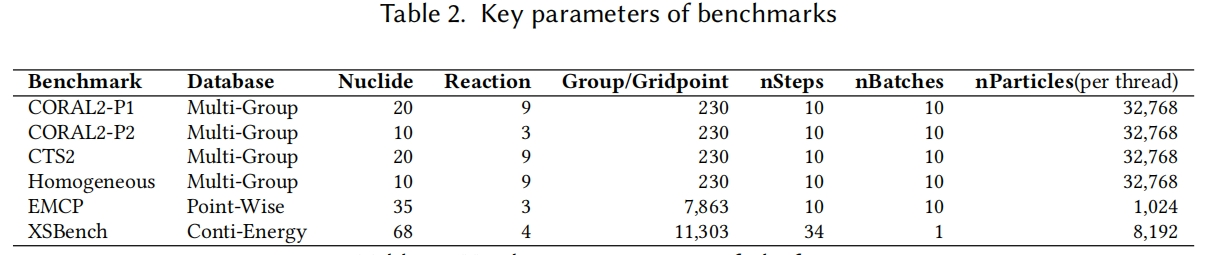
\includegraphics[width=0.9\textwidth]{figures/O-tab2.png}}
\end{figure}
\end{minipage}\par\medskip

\par\noindent\begin{minipage}{\linewidth}
\excerptlabel{Revised (Table~4, page 14):}\par
% Revised manuscript: Table 4
\begin{figure}[H]
  \centering
  \fbox{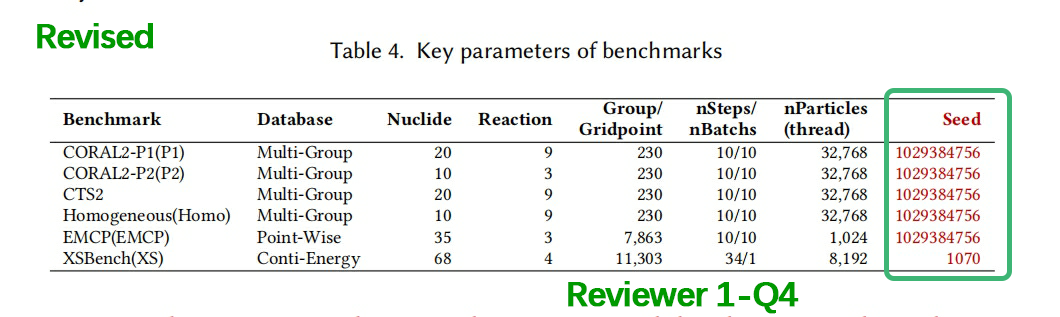
\includegraphics[width=0.9\textwidth]{news/R1-Q4-tab4.png}}
\end{figure}
\end{minipage}\par\medskip


\subsection{Question 5}
\begin{reviewcomment}
The authors describe how they measured the power for FluxArch but not for the baseline architectures. It is important to include such details for reproducibility and to ensure fair comparison (check the next cogent for the fairness).
\end{reviewcomment}

The CPU and GPU baselines run natively, whereas \name\ is evaluated through gem5 with McPAT and CACTI package-power modeling. We expanded the methodology to identify the measurement tools and align the accounting boundaries: \texttt{powerstat} records CPU/FT package power, \texttt{nvidia-smi} records GPU-board power, and off-package DDR5 is modeled separately where telemetry does not include it. This treatment includes co-packaged DDR4 or HBM only once and avoids omitting external DDR5 from the other platforms.

\revisionlocation{The native measurement tools, simulated power model, and measurement interval are specified in \textbf{Section 6.1}.}

\excerptlabel{Added (Section 6.1, page 14):}\par
\begin{manuscriptexcerpt}
\redsentence{\textbf{Power and Area Modeling Methodology}.} \redsentence{Table~5(b) distinguishes the measured and simulated platforms and defines the power-accounting boundary.} \redsentence{We execute all baselines natively.} \redsentence{For \intel, \amd, and \ft, we collect on-package power with \texttt{powerstat}~\papercite{powerstat}; for \ampare\ and \hopper, we record GPU-board power with \texttt{nvidia-smi}~\papercite{nvidia_smi}.} \redsentence{We report the mean power observed during each workload's timed execution region.} \redsentence{\name\ is evaluated in gem5, with package power modeled using McPAT and CACTI.}
\end{manuscriptexcerpt}
\begin{excerptreferences}
\paperreference{powerstat}
\paperreference{nvidia_smi}
\end{excerptreferences}

\par\noindent\begin{minipage}{\linewidth}
\revisionlocation{The platform-specific measurement and power-accounting boundaries are clarified in \textbf{Table~5}, which corresponds to original \textbf{Table~3}. Panel (a) revises the platform specifications, while panel (b) adds the evaluation methods and power-accounting boundaries.}

\excerptlabel{Original (Table~3, page 14):}\par
% Original manuscript: Table 3
\begin{figure}[H]
  \centering
  \fbox{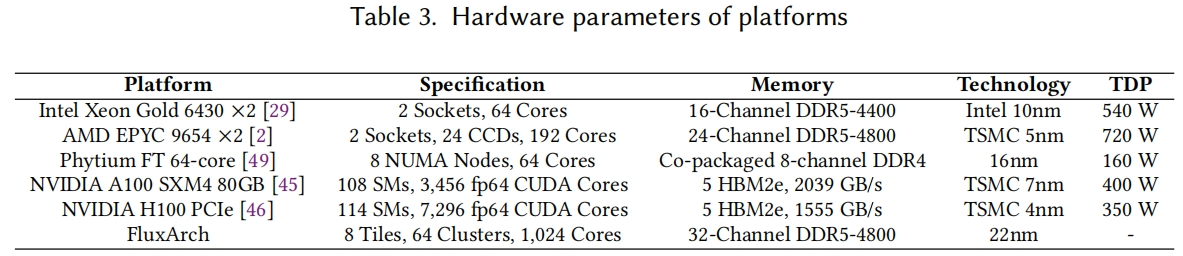
\includegraphics[width=0.9\textwidth]{figures/O-tab3.png}}
\end{figure}
\end{minipage}\par\medskip

\par\noindent\begin{minipage}{\linewidth}
\excerptlabel{Revised (Table~5, page 15):}\par
% Revised manuscript: Table 5
\begin{figure}[H]
  \centering
  \fbox{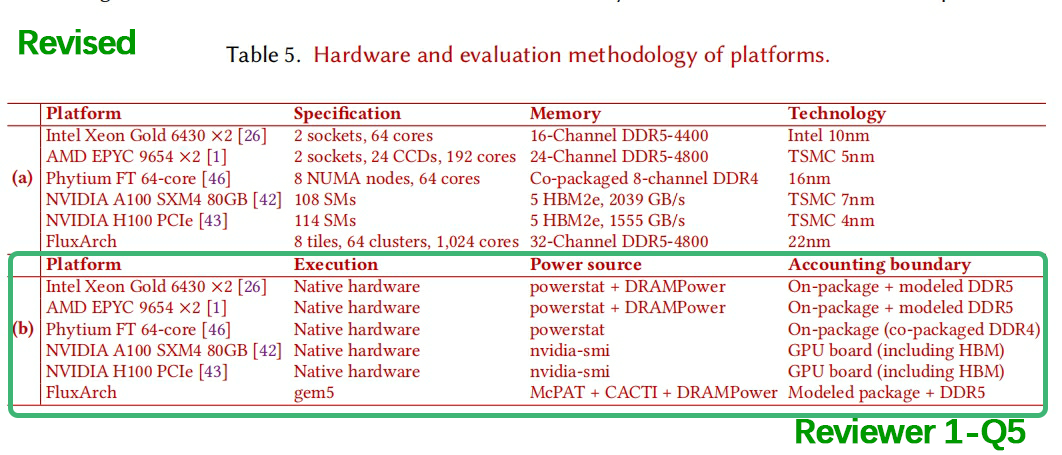
\includegraphics[width=0.9\textwidth]{news/R1-Q5-tab5.png}}
\end{figure}
\end{minipage}\par\medskip

\subsection{Question 6}
\begin{reviewcomment}
The authors mention that all reported energy metrics focus exclusively on on-chip power and that off-chip DRAM power is excluded. However, this makes the energy comparisons not very informative and, in cases, unfair. This is especially the case when comparing against architectures that have L3 cache. As FluxArch has no shared L3 cache, it is likely to have more misses than the baselines with L3 cache. Moreover, the baselines with L3 cache get unfairly penalized as their L3 power is included.
\end{reviewcomment}

We agree that on-chip-only energy accounting can bias a memory-bound comparison, especially when the platforms expose different memory-packaging boundaries. We therefore changed the evaluation to include co-packaged DDR4/HBM through device telemetry and off-package DDR5 through a common traffic-based DRAMPower~\papercite{drampower} model, with a $0.5\times$--$2\times$ sensitivity range for the modeled component. After this correction, the conservative process-scaled geometric-mean DRAM-inclusive energy-efficiency advantage remains 1.77$\times$ over H100 and 6.65$\times$ over Intel.

We now explain the choice of the $0.5\times$--$2\times$ range in \textbf{Section 6.1}. Ghose et al.~\papercite{ghose2018vampire} measured DDR3L read currents averaging 54.1\% below datasheet values for one vendor and data-pattern-dependent read-power differences of up to 91.6\%. Shi et al.~\papercite{shi2025drampower} report that DDR4 calibration reduced DRAMPower energy estimates by roughly half for most evaluated SPEC2006 workloads. These results motivate testing sizable modeling discrepancies, but do not establish an error bound for our DDR5 configuration. We therefore select reciprocal factors of 0.5 and 2 to test both overestimation and underestimation, with package power fixed; the range is a sensitivity-analysis choice, not a statistical confidence interval.

For process-scaled energy-efficiency bounds, we independently vary only the scaled FluxArch package power by $\pm30\%$ and each modeled off-package DRAM component over $0.5\times$--$2\times$, while keeping throughput and measured baseline package power fixed. We recompute the performance/W ratio at every endpoint combination and report its minimum and maximum; external DRAM power is not subject to process-node scaling or its 30\% margin.


\revisionlocation{The power-accounting boundary is revised in \textbf{Section 6.1} to include DRAM consistently across platforms.}

\excerptlabel{Revised (Section 6.1, page 14):}\par
\begin{manuscriptexcerpt}
\redsentence{We report DRAM-inclusive system power and energy.} \redsentence{Package power includes cores, caches, NoCs, and integrated memory controllers; for \ft, \ampare, and \hopper, the main memory is co-packaged (DDR4 or HBM) and is consequently covered by platform-level package/device telemetry.} \redsentence{In contrast, the DDR5 DIMMs of \intel\ and \amd, and the DDR5 channels assumed for \name, are physically off-package and are not covered by package-power readings.} \redsentence{We therefore add a separately modeled DRAM component to these platforms, avoiding asymmetric accounting that would include HBM/DDR4 power for the co-packaged-memory platforms but omit DDR5 power for the other platforms.}

\end{manuscriptexcerpt}

\revisionlocation{The traffic-based DRAM model and factor-of-two sensitivity analysis are added in \textbf{Section 6.1}.}

\excerptlabel{Added (Section 6.1, pages 14--15):}\par
\begin{manuscriptexcerpt}
\redsentence{For the DRAM model, we use DRAMPower 5~\papercite{drampower} with DDR5 timing and worst-case current parameters from the JEDEC DDR5 standard~\papercite{jedec_ddr5} and the Micron MT60B2G8HB-48B DDR5-4800 x8 datasheet~\papercite{micron_ddr5}.} \redsentence{\name\ is modeled with 32 single-rank DDR5-4800 channels, each containing eight x8 DRAM devices.} \redsentence{The model includes active-standby background power, refresh power, and read/write transfer power.} \redsentence{The external-memory energy of \intel\ and \amd\ is estimated using the same traffic-based DDR5 model and workload-specific memory traffic.}

\redsentence{Because the simulation does not expose DRAM command traces or row-buffer events, we use a traffic-based DRAM energy estimate rather than claiming command-level precision.} \redsentence{For each \name\ workload, we derive read/write traffic from the memory-system statistics and use the simulated execution time.} \redsentence{Prior DRAM measurement and calibration studies report substantial discrepancies between datasheet-based estimates and measured consumption~\papercite{ghose2018vampire,shi2025drampower}.} \redsentence{Motivated by these findings, we select a $0.5\times$--$2\times$ range for the nominal modeled DRAM power of every off-package DDR5 platform (\intel, \amd, and \name).} \redsentence{This range is a sensitivity-analysis choice, not an empirically established DDR5 error bound or a statistical confidence interval.}
\end{manuscriptexcerpt}
\begin{excerptreferences}
\paperreference{drampower}
\paperreference{jedec_ddr5}
\paperreference{micron_ddr5}
\paperreference{ghose2018vampire}
\paperreference{shi2025drampower}
\end{excerptreferences}

\revisionlocation{The energy-efficiency comparison and conservative lower bounds are updated in \textbf{Section 6.2} to include DRAM power.}

\excerptlabel{Original (Section 6.2, pages 14--15):}\par
\begin{manuscriptexcerpt}
\graysentence{\textbf{Iso-Process Energy Efficiency}.} \graysentence{As shown in Fig.~13(b), the energy efficiency advantage is even more pronounced.} \graysentence{By comparing projected iso-process nodes, we isolate the architectural contributions.} \graysentence{According to Section. 6.1, the power projection error is 30\%.} \graysentence{Therefore, we incorporate this margin into our energy efficiency evaluation, which is represented as error bars in our results.} \graysentence{Without the workload orchestration, the energy efficiency of \name, mainstream server CPUs and high-end GPUs is at odds with each other.} \graysentence{With the orchestration enabled, optimizing data locality and minimizing cross-tile traffic, \name\ demonstrates a superior geometric mean energy efficiency improvement from \textbf{3.98}$\boldsymbol{\times}$ (vs. \ft, 5.69$\times$ discounted by 30\%) to \textbf{9.84}$\boldsymbol{\times}$ (vs. \intel, 14.06$\times$ discounted by 30\%) even accounting for the potential projection error of pessimistic assumption.} \graysentence{We also report the energy efficiency of the raw, unscaled data based on the 22 nm technology node.} \graysentence{Even in this case, \name\ still achieves an energy efficiency improvement of 1.17$\times$ (vs. \hopper) to 4.59$\times$ (vs. \intel).}
\end{manuscriptexcerpt}

\excerptlabel{Revised (Section 6.2, pages 15--16):}\par
\begin{manuscriptexcerpt}
\redsentence{\textbf{DRAM-Inclusive Energy Efficiency}.} \redsentence{Fig.~13(c,d) reports DRAM-inclusive power and energy efficiency under the sensitivity bounds defined in Section 6.1.} \redsentence{Process-scaled results separate architectural effects from process scaling while accounting consistently for external memory.}

\redsentence{In the process-scaled comparison, \name\ improves geometric-mean DRAM-inclusive efficiency by \textbf{2.85}$\boldsymbol{\times}$ over \hopper\ to \textbf{10.58}$\boldsymbol{\times}$ over \intel.}

\redsentence{The sensitivity analysis preserves the process-scaled conclusion: across the combined DRAM and technology-scaling bounds, the geometric-mean improvement with orchestration remains 1.77$\times$ over \hopper\ and 6.65$\times$ over \intel\ at the conservative lower bound.}

\end{manuscriptexcerpt}

\par\noindent\begin{minipage}{\linewidth}
\revisionlocation{The power breakdown and energy-efficiency plots are updated in \textbf{Figure~13(c,d)} to include DRAM power and the corresponding sensitivity bounds. Panel (c) is newly added; panel (d) revises the original energy-efficiency plot.}

\excerptlabel{Original (Figure~13, page 15):}\par
% Original manuscript: Figure 13
\begin{figure}[H]
  \centering
  \fbox{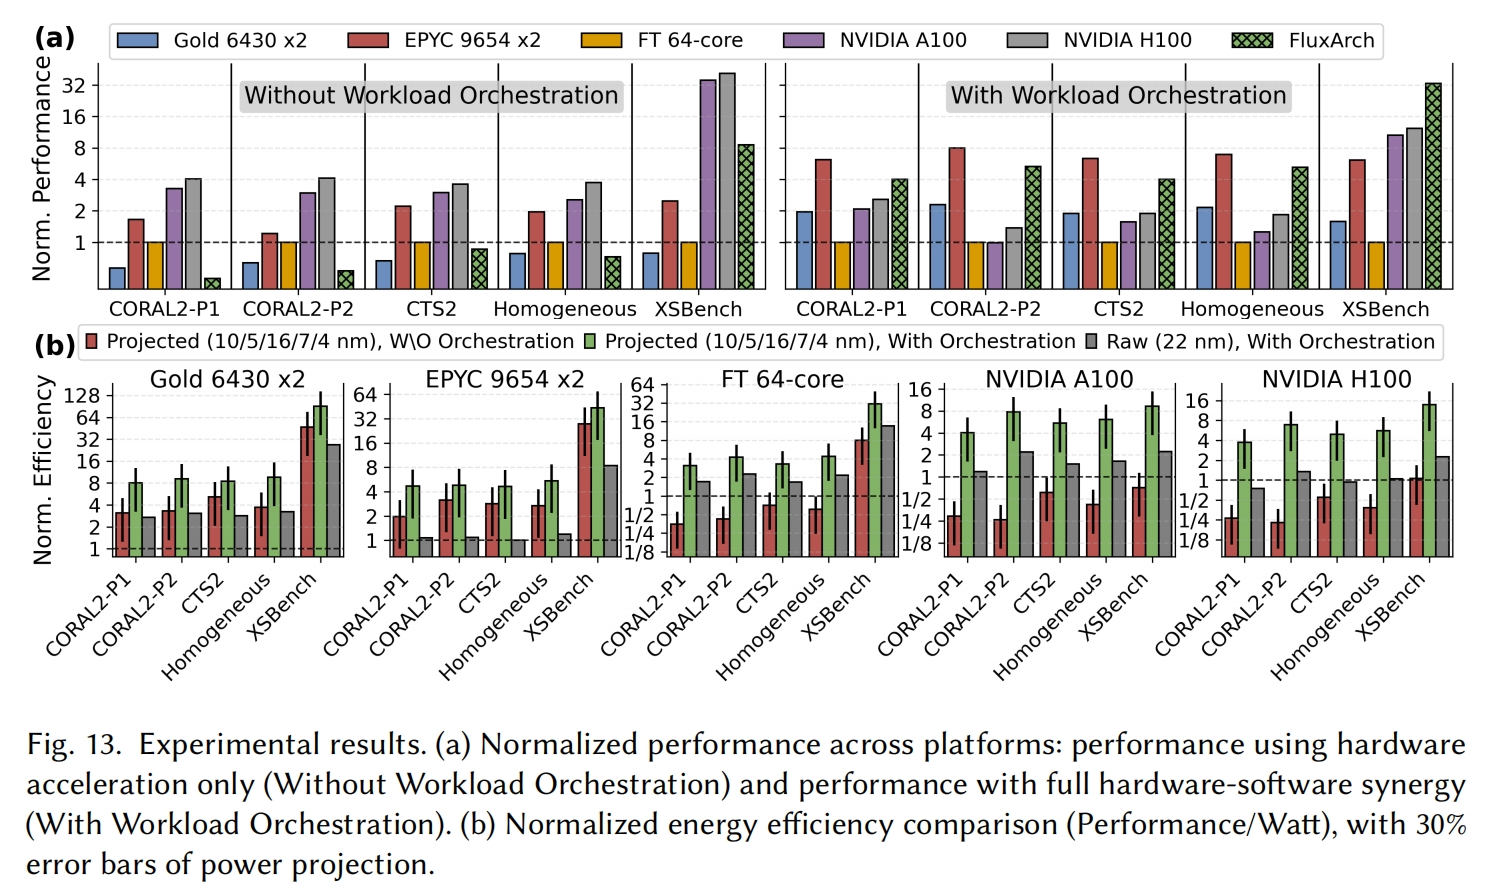
\includegraphics[width=0.9\textwidth]{figures/O-fig13.png}}
\end{figure}
\end{minipage}\par\medskip

\par\noindent\begin{minipage}{\linewidth}
\excerptlabel{Revised (Figure~13, page 16):}\par
% Revised manuscript: Figure 13
\begin{figure}[H]
  \centering
  \fbox{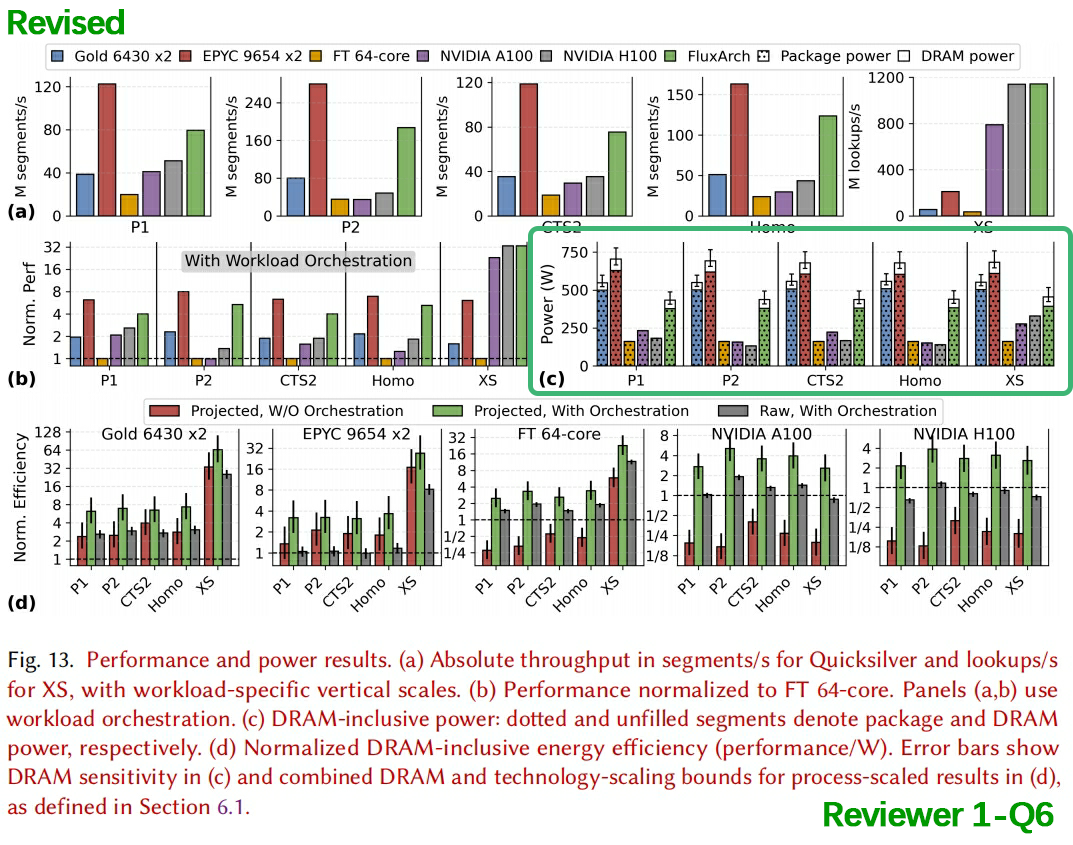
\includegraphics[width=0.9\textwidth]{news/R1-Q6-fig13.png}}
\end{figure}
\end{minipage}\par\medskip


\subsection{Question 7}
\begin{reviewcomment}
In Section 6.6 on scalability evaluation, the authors argue that the Gold 6430 $\times$2 and FT 64-core outperform the proposed approach because their monolithic LLCs provide a unified, low-latency shared memory space that enables efficient inter-thread synchronization at lower core counts. However, no empirical data is provided to support this claim. Do the authors have measurements or analysis validating this explanation? This is particularly important since both systems significantly outperform FluxArch in most cases, and no experiments beyond 64 cores are possible to demonstrate whether FluxArch would eventually surpass them at larger scales (as they have no more cores).
\end{reviewcomment}

We do not have controlled measurements that isolate LLC organization as the cause of the observed scaling difference. Cache organization, memory hierarchy, core microarchitecture, and synchronization overhead vary together across the evaluated platforms. The commercial baseline systems expose tightly coupled hardware configurations that cannot be independently reconfigured to change only LLC organization while holding the other factors constant. Our measurements therefore do not support the earlier LLC-based causal explanation, which we have removed. The revised discussion reports only the observed scaling trends within the evaluated ranges, without extrapolating Intel or FT beyond 64 cores.


\revisionlocation{The scaling discussion is revised in \textbf{Section 6.6} to distinguish the measured trends from an unisolated LLC-based explanation and limit the CPU comparison to the evaluated range.}

\excerptlabel{Original (Section 6.6, page 17):}\par
\begin{manuscriptexcerpt}
\graysentence{Fig.~17 evaluates the scaling efficiency of \name\ against three CPU platforms.} \graysentence{In the small-scale regime ($<64$ cores), \name\ and \amd\ exhibit low efficiency.} \graysentence{This is attributed to the architectural trade-off between monolithic and distributed Last-Level Caches (LLCs).} \graysentence{Monolithic LLCs (\intel/\ft) provide a unified, low-latency shared memory pool that excels at handling inter-thread synchronization with a low core count.} \graysentence{Conversely, the distributed LLCs in \name\ and \amd\ incur higher coherence overhead when the workload is concentrated in fewer cores, as the shared memory programming model imposes a latency barrier on cross-cluster communication.} \graysentence{However, in the large-scale regime ($>64$ cores), \name's hierarchical design demonstrates superior efficiency, surpassing \amd\ across nearly all benchmarks as the system scales.}
\end{manuscriptexcerpt}

\excerptlabel{Revised (Section 6.6, page 20):}\par
\begin{manuscriptexcerpt}
\redsentence{\textbf{System-Level Scalability.}} \redsentence{Fig.~18 evaluates the scaling efficiency of \name\ against three CPU platforms.} \redsentence{At up to 64 cores, \intel\ and \ft\ retain higher scaling efficiency than \name\ for most workloads.} \redsentence{Cache organization, memory hierarchy, core microarchitecture, and synchronization overhead vary jointly across these platforms.} \redsentence{The commercial baselines do not provide otherwise identical configurations differing only in LLC organization, so this cross-platform comparison characterizes system-level scaling rather than the isolated effect of LLC design.} \redsentence{The evaluated \intel\ and \ft\ configurations cover at most 64 cores, limiting the comparison to this range.} \redsentence{Within the measured range, \name\ continues scaling to 1,024 cores and exceeds the measured \amd\ scaling efficiency across nearly all workloads at larger core counts.}
\end{manuscriptexcerpt}

\par\noindent\begin{minipage}{\linewidth}
\excerptlabel{Figure~18 (page 20):}\par
% Manuscript: Figure 18
\begin{figure}[H]
  \centering
  \fbox{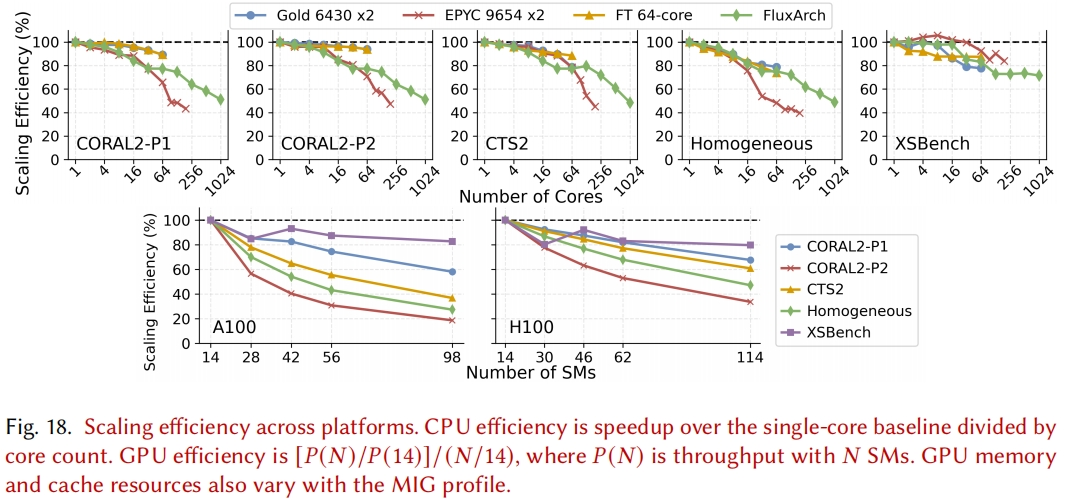
\includegraphics[width=0.9\textwidth]{figures/fig18.png}}
\end{figure}
\end{minipage}\par\medskip


\subsection{Question 8}
\begin{reviewcomment}
Why are no scalability results presented for GPUs? There are different ways to limit the GPU usage and emulate scalability. The authors are recommended to add such results or provide good reasons not to.
\end{reviewcomment}

We added GPU scaling measurements by fixing each workload's problem size and increasing the number of streaming multiprocessors (SMs) assigned to one GPU instance through NVIDIA Multi-Instance GPU (MIG). The five profiles provide 14, 28, 42, 56, and 98 SMs on A100, and 14, 30, 46, 62, and 114 SMs on H100. Each workload runs on one instance at a time. Efficiency is $E(N)=[P(N)/P(14)]/(N/14)$, where $P(N)$ is throughput with $N$ SMs. Because memory capacity, cache, and memory bandwidth also depend on the profile, these results characterize scaling across GPU resource configurations. At 98 SMs on A100 and 114 SMs on H100, efficiency ranges from 18.62\% to 82.73\% and from 33.65\% to 79.65\%, respectively; XSBench scales best and CORAL2-P2 scales least efficiently on both GPUs.

\revisionlocation{The MIG allocation method, normalization, and GPU scaling trends are described in \textbf{Section 6.6}.}

\excerptlabel{Added (Section 6.6, page 20):}\par
\begin{manuscriptexcerpt}
\redsentence{We additionally evaluate GPU scaling by keeping each workload's problem size fixed and increasing the number of streaming multiprocessors (SMs) assigned to one GPU instance. NVIDIA Multi-Instance GPU (MIG) partitions a physical GPU into isolated instances with dedicated compute and memory resources. We use five MIG profiles to allocate 14--98 SMs on \ampare, and 14--114 SMs on \hopper. The cache and memory-bandwidth allocations vary with the profile, so these measurements reflect scaling across GPU resource configurations. At 98 SMs on \ampare\ and 114 SMs on \hopper, efficiency ranges from 18.62\% to 82.73\% and from 33.65\% to 79.65\%, respectively. XSBench scales best on both GPUs, while CORAL2-P2 scales least efficiently.}
\end{manuscriptexcerpt}

\par\noindent\begin{minipage}{\linewidth}
\revisionlocation{The GPU scaling results are added in \textbf{Figure~18}, with GPU scale labeled by the actual SM counts. The CPU panels are revised from the original figure, while the GPU panels are newly added.}

\excerptlabel{Revised (Figure~18, page 20):}\par
% Revised manuscript: Figure 18
\begin{figure}[H]
  \centering
  \fbox{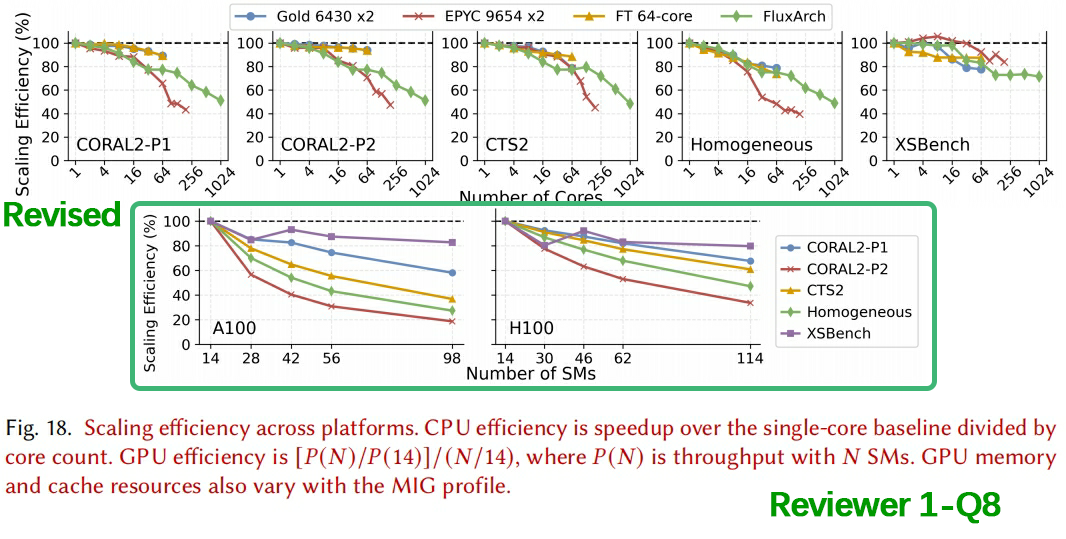
\includegraphics[width=0.9\textwidth]{news/R1-Q8-fig18.png}}
\end{figure}
\end{minipage}\par\medskip

\subsection{Question 9}
\begin{reviewcomment}
The scalability behaviour of the XSBench benchmark is an outlier. The authors are recommended to discuss the reason behind this. Are there certain generalizable characteristics in this benchmark that affect FluxArch and EPYC scaling?
\end{reviewcomment}

We revised \textbf{Figure~18} for clarity and aligned the y-axis scales across panels.

XSBench is an outlier in the favorable direction: it retains approximately 71\% scaling efficiency at 1,024 cores, compared with approximately 48\%--52\% for the other \name\ workloads. On EPYC, XSBench similarly retains approximately 84\% efficiency at 192 cores, compared with approximately 40\%--47\% for the four Quicksilver workloads. EPYC and \name\ both organize cores into local cache-sharing groups---CCDs sharing L3 and clusters sharing L2, respectively. Under our LLC-aware process mapping, XSBench's independent lookups require no inter-rank particle-state exchange as execution expands across these groups, unlike Quicksilver. This favorable scaling does not imply full cache residency: its 241-MiB database exceeds the 4-MiB cluster L2 on \name, and the \name\ measurements in Table~6(a) report the lowest L2 read hit rate and highest normalized DRAM read traffic among the evaluated workloads. We clarified this shared workload characteristic and its relationship to the two platforms' cache-sharing groups in \textbf{Section 6.6}.


\par\noindent\begin{minipage}{\linewidth}
\excerptlabel{Original (Figure~17, page 18):}\par
% Original manuscript: Figure 17
\begin{figure}[H]
  \centering
  \fbox{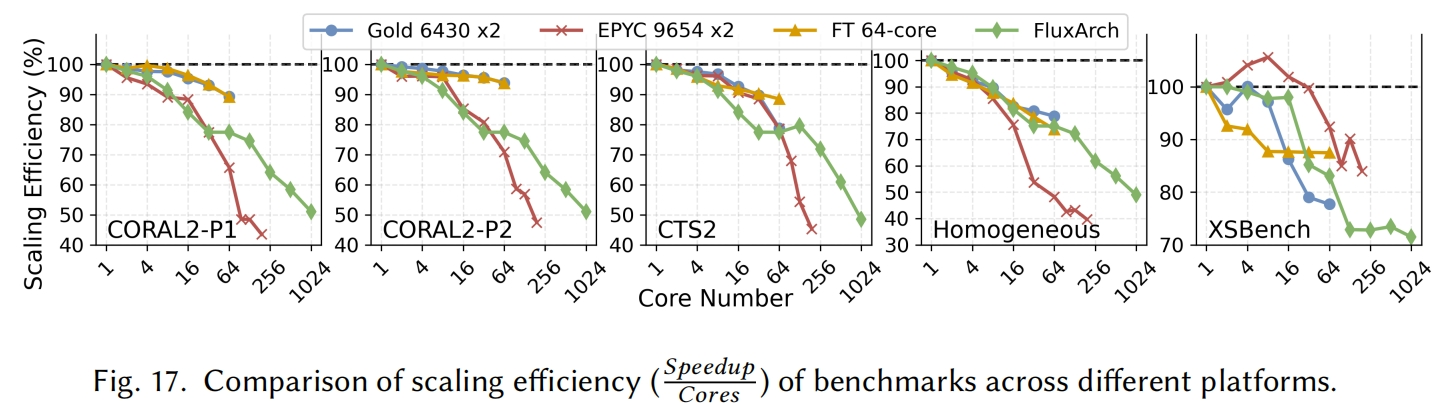
\includegraphics[width=0.9\textwidth]{figures/O-fig17.png}}
\end{figure}
\end{minipage}\par\medskip

\par\noindent\begin{minipage}{\linewidth}
\excerptlabel{Revised (Figure~18, page 20):}\par
% Revised manuscript: Figure 18
\begin{figure}[H]
  \centering
  \fbox{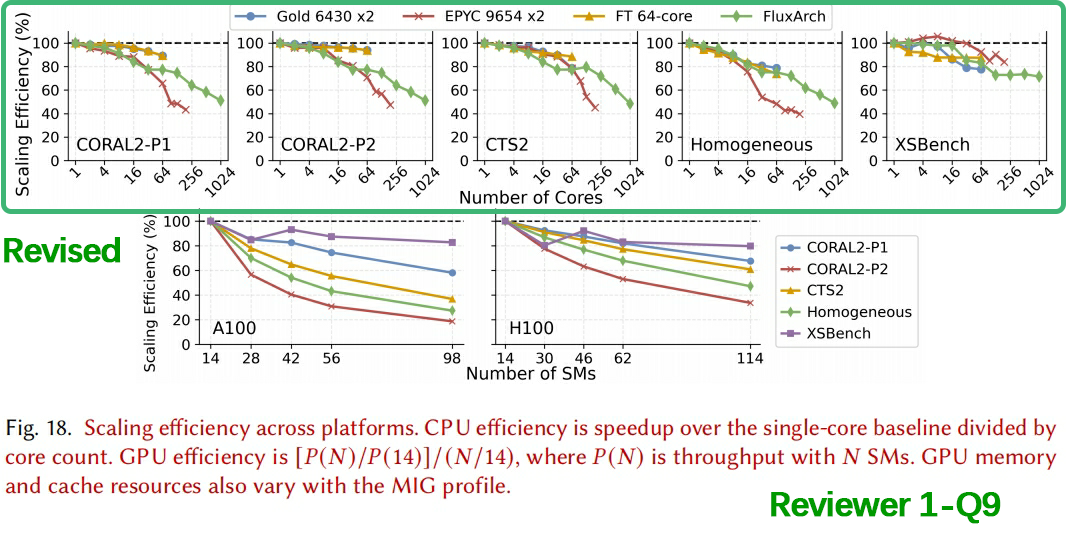
\includegraphics[width=0.9\textwidth]{news/R1-Q9-fig18.png}}
\end{figure}
\end{minipage}\par\medskip



\revisionlocation{The favorable XSBench scaling is explained in \textbf{Section 6.6} through its independent lookups and absence of inter-rank particle exchange.}

\excerptlabel{Added (Section 6.6, page 20):}\par
\begin{manuscriptexcerpt}
\redsentence{XSBench retains approximately 71\% scaling efficiency at 1,024 cores, compared with approximately 48\%--52\% for the other \name\ workloads.} \redsentence{EPYC and \name\ both organize cores into local cache-sharing groups---CCDs sharing L3 and clusters sharing L2, respectively.} \redsentence{Under our LLC-aware process mapping, XSBench's independent lookups require no inter-rank particle-state exchange as execution expands across these groups, unlike Quicksilver.} \redsentence{This favorable scaling does not imply full cache residency: the \name\ measurements in Table~6(a) show that XSBench has the largest database, the lowest L2 read hit rate, and the highest normalized DRAM read traffic among the evaluated workloads.}
\end{manuscriptexcerpt}

\revisionlocation{The discussion also relates this behavior to the memory measurements in \textbf{Table~6(a)}.}
\par\noindent\begin{minipage}{\linewidth}
\excerptlabel{Added (Table~6(a), page 18):}\par
% Revised manuscript: Figure 6(a)
\begin{figure}[H]
  \centering
  \fbox{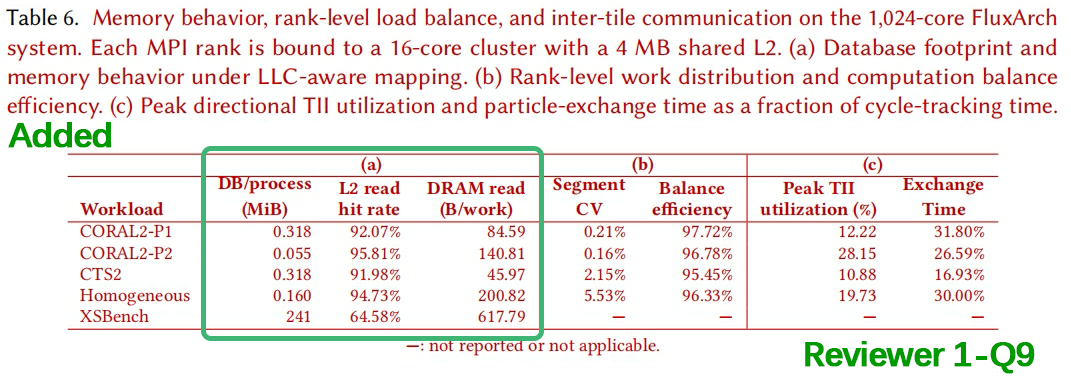
\includegraphics[width=0.9\textwidth]{news/R1-Q9-tab6a.png}}
\end{figure}
\end{minipage}\par\medskip

\subsection{Question 10}
\begin{reviewcomment}
The authors primarily evaluate CPUs and GPUs, but do not discuss alternative architectures such as FPGAs, CGRAs, or specialized manycore systems like Graphcore. These platforms may help mitigate some of the bottlenecks identified for CPUs and GPUs. In addition, prior work has explored FPGA-based approaches for Monte Carlo simulations. A comparison (discussion, not necessarily a complete evaluation) would strengthen the paper and provide a more complete perspective on the proposed architecture's position in the design space.
\end{reviewcomment}

We agree that FPGA-based Monte Carlo transport acceleration is relevant prior work and was insufficiently discussed in the original manuscript. We now explicitly discuss Gokhale et al.'s FPGA pipeline for ray--surface intersection in Monte Carlo radiative heat transfer and Luu et al.'s FPGA implementation of MCML photon transport. The comparison in \textbf{Section 8} is anchored in the boundary of specialization: these works specialize a transport loop or a particular photon-transport pipeline, whereas \name\ retains instruction-driven MIMD transport control and integrates selected FP64 arithmetic kernels into each core. Their application-specific datapaths do not establish the cache/DRAM and communication organization used here for database-intensive neutron transport. We explain how \name\ combines core-local acceleration with shared-cache reuse and topology-aware MPI/OpenMP orchestration, rather than suggesting that FPGAs cannot handle stochastic control. We also distinguish CGRA spatial mapping from instruction-driven control and Graphcore's tile-local memory/exchange organization from \name's cache/DRAM hierarchy. The discussion compares design choices, not speedup values obtained under different physical models and workloads.

\revisionlocation{The architectural differences from FPGAs, CGRAs, and the Graphcore IPU, together with the limits of a quantitative comparison, are clarified in \textbf{Section 8}.}

\excerptlabel{Added (Section 8, pages 22--23):}\par
\begin{manuscriptexcerpt}
\redsentence{\textbf{Alternative Programmable Architectures.}} \redsentence{Gokhale et al.~\papercite{gokhale2004radiative} accelerate Monte Carlo radiative heat transfer with an FPGA ray--surface intersection pipeline; Luu et al.~\papercite{luu2009mcml} implement MCML photon transport through multilayer tissue as a dedicated FPGA pipeline.} \redsentence{The distinction is the boundary of specialization: these designs specialize a transport loop or photon-transport pipeline, whereas \name\ retains instruction-driven MIMD transport control and specializes selected FP64 arithmetic kernels within each core.} \redsentence{Their datapaths target the geometry and interaction models of their respective applications.} \redsentence{\name\ couples its core-local Engines with cache- and DRAM-backed database access and topology-aware MPI/OpenMP orchestration, addressing data reuse and inter-process communication alongside arithmetic acceleration.} \redsentence{CGRAs likewise expose configurable spatial datapaths, with computation mapped onto processing elements and their interconnect~\papercite{cgra-survey}; \name\ instead leaves dynamic transport control in programmable cores.} \redsentence{The Graphcore IPU is also MIMD, but its tile-local memory and explicit exchange~\papercite{ipu-particle-physics} contrast with \name's cache/DRAM hierarchy and core-local Engine.} \redsentence{Differences in physical models, workloads, and evaluation conditions preclude a direct comparison of the cited speedup values.}
\end{manuscriptexcerpt}
\begin{excerptreferences}
\paperreference{gokhale2004radiative}
\paperreference{luu2009mcml}
\paperreference{cgra-survey}
\paperreference{ipu-particle-physics}
\end{excerptreferences}

\subsection{Question 11}
\begin{reviewcomment}
The authors mentioned related architectures are using specialized, area-efficient designs (Fu et al [22] and Zhang et al. [72]). However, there is no comparison with these approaches. In the related work section, the authors mention briefly how FluxArch qualitatively improves over these works but do not provide any quantitative comparisons. The authors are recommended to include a more detailed comparison against the mentioned approaches as this would strengthen the work considerably.
\end{reviewcomment}

Fu et al. and Zhang et al. propose the specialized MCPT architectures most closely related to \name. We added a detailed comparison in \textbf{Table~7}, covering core design, hierarchy and system scale, cache and memory organization, evaluation methodology, workloads, and the quantitative results reported by each work.

We also explain in \textbf{Section 8} why these published values cannot be compared directly. Fu et al. report performance, performance/W, and performance/area relative to a modeled four-core Cortex-A15 system; Zhang et al. report scaling efficiency relative to their own single-core configuration. \name's performance and energy-efficiency ratios instead use our CPU/GPU baselines. Workload inputs, system resources, and accounting boundaries also differ substantially. The table therefore preserves each result's original baseline rather than converting these values into cross-architecture speedups.

Reimplementing the designs in a common framework would not, by itself, establish a fair comparison. Although the papers provide major architectural parameters, their descriptions do not fully specify all implementation and modeling choices needed for a unified evaluation. In particular, Zhang et al. do not report a process node or a power/area model. Reconstructing customized simulator configurations and adding missing power/area models would require assumptions that could affect the results and confound architectural differences with reconstruction choices.

\revisionlocation{The comparison with Fu et al. and Zhang et al. is revised in \textbf{Section 8} to clarify the architectural differences.}

\excerptlabel{Original (Section 8, page 19):}\par
\begin{manuscriptexcerpt}
\graysentence{Recent microarchitectural studies have shifted toward specialized, area-efficient designs.} \graysentence{Fu et al. pioneered the use of clustered small cores to improve energy-to-area ratios for MCPT workloads, a foundation subsequently extended by Zhang et al. to a 128-core cluster with optimized parallelization.} \graysentence{Our \name\ system achieves a significant leap forward by: (1) scaling the architecture to 1,024 cores using a hierarchical chiplet-based design; (2) integrating a dedicated execution engine to offload dominant kernels; and (3) proposing a topology-aware hardware-software co-design that transcends the scalability limits of prior clustered small-core architectures.}
\end{manuscriptexcerpt}

\excerptlabel{Revised (Section 8, page 22):}\par
\begin{manuscriptexcerpt}
\redsentence{\textbf{Specialized MCPT Architectures.}} \graysentence{Recent microarchitectural studies have shifted toward specialized, area-efficient designs.} \redsentence{Table~7 compares \name\ with Fu et al.~\papercite{minimctad} and Zhang et al.~\papercite{128mc} in core design, hierarchy, cache and memory organization, evaluation methodology, workloads, and author-reported results.} \redsentence{Fu et al. use simplified in-order cores to improve area and power efficiency, while Zhang et al. scale to 128 cores through 32-core cache-sharing clusters and OpenMP dynamic scheduling.} \redsentence{\name\ combines a 1,024-core hierarchy with a core-local Engine and topology-aware spatial mapping.}

\end{manuscriptexcerpt}
\begin{excerptreferences}
\paperreference{minimctad}
\paperreference{128mc}
\end{excerptreferences}

\revisionlocation{The limits of comparing published results and reconstructing prior designs fairly are added in \textbf{Section 8}.}

\excerptlabel{Added (Section 8, page 22):}\par
\begin{manuscriptexcerpt}
\redsentence{The reported results use substantially different experimental conditions, including workload inputs, core counts, cache and memory configurations, reference baselines, and power-accounting boundaries.} \redsentence{Fu et al. report performance, performance/W, and performance/area relative to a modeled four-core Cortex-A15 system.} \redsentence{Zhang et al. report scaling efficiency relative to their own single-core configuration.} \redsentence{\name's performance and energy-efficiency ratios use the evaluated CPU/GPU platforms as baselines, whereas its scaling efficiency is relative to one core.} \redsentence{Thus, Table~7 places each work's results in context rather than establishing cross-architecture speedups or an efficiency ranking.}

\redsentence{A unified reimplementation would also require resolving implementation and modeling choices not fully specified in the papers, rather than merely matching their listed hardware parameters.} \redsentence{In particular, Zhang et al. do not report a process node or a power/area model.} \redsentence{Reconstructing the customized simulator configurations and supplying missing power/area models would introduce additional assumptions that could affect the results, confounding architectural differences with reconstruction choices and weakening the fairness of a direct comparison.}


\end{manuscriptexcerpt}


\par\noindent\begin{minipage}{\linewidth}
\revisionlocation{The detailed architectural parameters and author-reported results, with their original comparison baselines, are added in \textbf{Table~7}.}

\excerptlabel{Added (Table~7, page 22):}\par
% Revised manuscript: Table 7
\begin{figure}[H]
  \centering
  \fbox{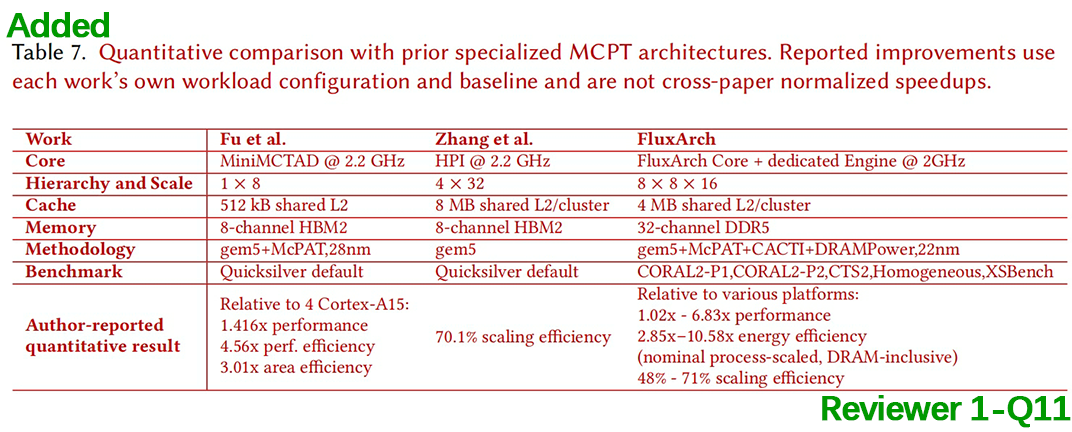
\includegraphics[width=0.9\textwidth]{news/R1-Q11-tab7.png}}
\end{figure}
\end{minipage}\par\medskip

\subsection{Question 12}
\begin{reviewcomment}
The authors are recommended to add references to the first paragraphs of the introduction for readers interested in more details.
\end{reviewcomment}

We sincerely thank you for your helpful and constructive suggestion. We added the corresponding references.


\revisionlocation{References supporting the introductory motivation and background claims are added in \textbf{Section 1}.}

\excerptlabel{Original (Section 1, page 1):}\par
\begin{manuscriptexcerpt}
\graysentence{Monte Carlo Particle Transport (MCPT) is the authoritative standard for simulating interactions between particles and material, widely applied in critical fields such as nuclear reactor safety and medical radiation therapy.} \graysentence{Its core philosophy involves performing independent and repeated random simulations of billions of particles and estimating macroscopic physical quantities, such as particle penetration probability and energy deposition distribution, based on statistical methods.} \graysentence{Since each particle is statistically independent, MCPT theoretically possesses rich parallel potential.}

\graysentence{However, in practice, each particle's transport is driven by random sampling, which determines its energy state, reaction type (e.g., fission, capture), and interaction position via probability distributions.} \graysentence{This stochastic nature renders particle execution paths highly unpredictable, thereby introducing extensive random control flow.} \graysentence{As particles propagate, they must frequently access multi-dimensional probability databases based on their current energy and reaction states to perform interpolation and physical calculations.} \graysentence{Since particles traverse highly dissimilar energy regions in state space, successive steps often access widely separated entries in the probability tables, resulting in significant spatial irregularity in memory access.}

\graysentence{Consequently, the MCPT workload simultaneously exhibits Massive Parallelism, Random Control Flow, and Irregular Memory Access---a combination of characteristics that poses extreme architectural challenges, resulting in severe architectural mismatches on modern general-purpose computing platforms.}
\end{manuscriptexcerpt}

\excerptlabel{Revised (Section 1, page 1):}\par
\begin{manuscriptexcerpt}
\redsentence{Monte Carlo Particle Transport (MCPT) is a widely used high-fidelity method for simulating interactions between particles and materials, with applications including nuclear reactor analysis and medical radiation treatment planning~\papercite{mcpt1,mcpt2,openmc,shift,review}.} \redsentence{Its core philosophy involves performing independent and repeated random simulations of billions of particle histories and estimating macroscopic physical quantities, such as particle penetration probability and energy deposition distributions, using statistical methods~\papercite{mcpt1,mcpt2}.} \redsentence{Since particle histories are statistically independent, MCPT theoretically possesses abundant parallelism~\papercite{mcpt-spec1,mcpt-spec3}.}

\graysentence{However, in practice, each particle's transport is driven by random sampling, which determines its energy state, reaction type (e.g., fission, capture), and interaction position via probability distributions.} \graysentence{This stochastic nature renders particle execution paths highly unpredictable, thereby introducing extensive random control flow.} \graysentence{As particles propagate, they must frequently access multi-dimensional probability databases based on their current energy and reaction states to perform interpolation and physical calculations.} \redsentence{Since particles traverse highly dissimilar energy regions in state space, successive steps often access widely separated entries in the probability tables, resulting in significant spatial irregularity in memory access~\papercite{mcpt-spec1,mcpt-spec2,mcpt-spec3}.}

\redsentence{Consequently, the MCPT workload simultaneously exhibits Massive Parallelism, Random Control Flow, and Irregular Memory Access---a combination of characteristics that poses substantial architectural challenges on modern general-purpose computing platforms~\papercite{mcpt-spec1,mcpt-spec2,mcpt-spec3}.}
\end{manuscriptexcerpt}
\begin{excerptreferences}
\paperreference{mcpt-spec3}
\paperreference{mcpt-spec1}
\paperreference{review}
\paperreference{mcpt1}
\paperreference{mcpt2}
\paperreference{mcpt-spec2}
\paperreference{shift}
\paperreference{openmc}
\end{excerptreferences}

\clearpage
\section{Reviewer 2}

\subsection{Question 1}
\begin{reviewcomment}
Clarify measured vs. simulated and validate the model. State whether each baseline is real hardware or gem5, and validate FluxArch against a fabricated reference---the headline 6.83$\times$/9.84$\times$ claims depend on this.
\end{reviewcomment}
We sincerely thank you for your helpful and constructive suggestion. We agree that the evaluation must distinguish native measurements from simulation and provide direct evidence for the modeled components.

\begin{enumerate}[label=(\arabic*)]
\setlength{\emergencystretch}{1em}
\item \textbf{Measured versus simulated results.} The Intel, AMD, FT, A100, and H100 baselines are executed and measured on native hardware, whereas \name\ performance is simulated in gem5 and its package power and area are modeled with McPAT and CACTI. We revised the platform description so that the measurement and modeling boundary is explicit for every platform. The native results are hardware measurements, while the \name\ results are calibrated simulation estimates.


\revisionlocation{The distinction between native measurements and modeled results is clarified in \textbf{Section 6.1}.

The platform-specific evaluation and power-accounting methods are specified in \textbf{Table~5}, replacing original \textbf{Table~3}. Panel (a) revises the platform specifications, while panel (b) adds the evaluation methods and power-accounting boundaries.}

\par\noindent\begin{minipage}{\linewidth}
\excerptlabel{Original (Table~3, page 14):}\par
% Original manuscript: Table 3
\begin{figure}[H]
  \centering
  \fbox{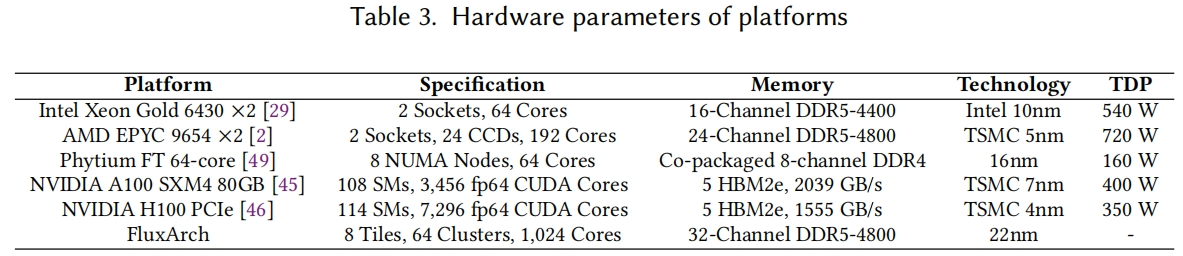
\includegraphics[width=0.9\textwidth]{figures/O-tab3.png}}
\end{figure}
\end{minipage}\par\medskip

\par\noindent\begin{minipage}{\linewidth}
\excerptlabel{Revised (Table~5, page 15):}\par
% Revised manuscript: Table 5
\begin{figure}[H]
  \centering
  \fbox{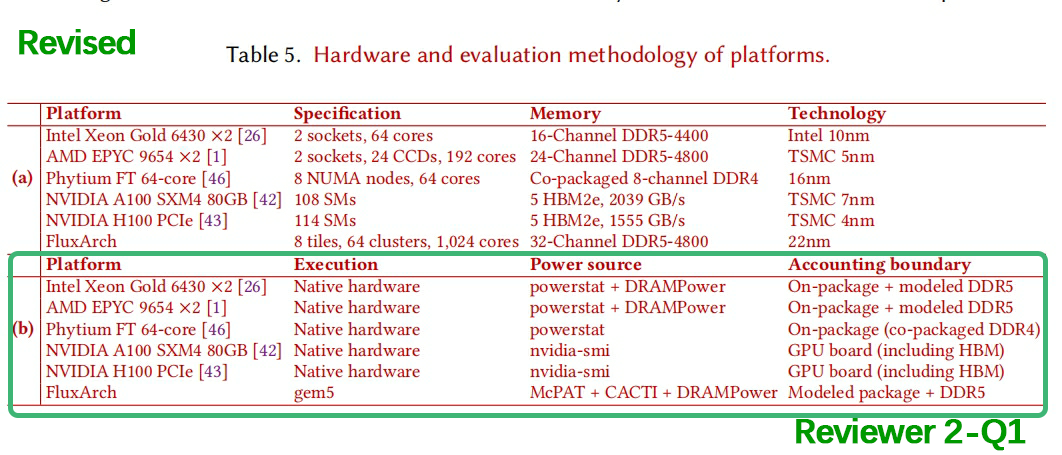
\includegraphics[width=0.9\textwidth]{news/R2-Q1-tab5.png}}
\end{figure}
\end{minipage}\par\medskip

\item \textbf{Model validation.} We added six controlled comparisons against RK3562 Cortex-A53 silicon for the core and cache/DRAM paths and derived Engine latency directly from fixed-latency RTL operators and loop bounds. The silicon comparison yields matching checksums, 6.7\% mean absolute percentage error, and 13.5\% maximum absolute percentage error; the Engine expression is derived from the implementation. This establishes implementation traceability, not an independent statistical calibration between two timing models. We describe these results as calibrated simulation evidence while clearly retaining the limitation that the complete 1,024-core system has not been fabricated.

\revisionlocation{The deterministic Engine latency is derived from RTL operator timing and loop bounds in \textbf{Section 4.2}.}

\par\noindent\begin{minipage}{\linewidth}
\excerptlabel{Figure~9 (page 9):}\par
% Manuscript: Figure 9
\begin{figure}[H]
  \centering
  \fbox{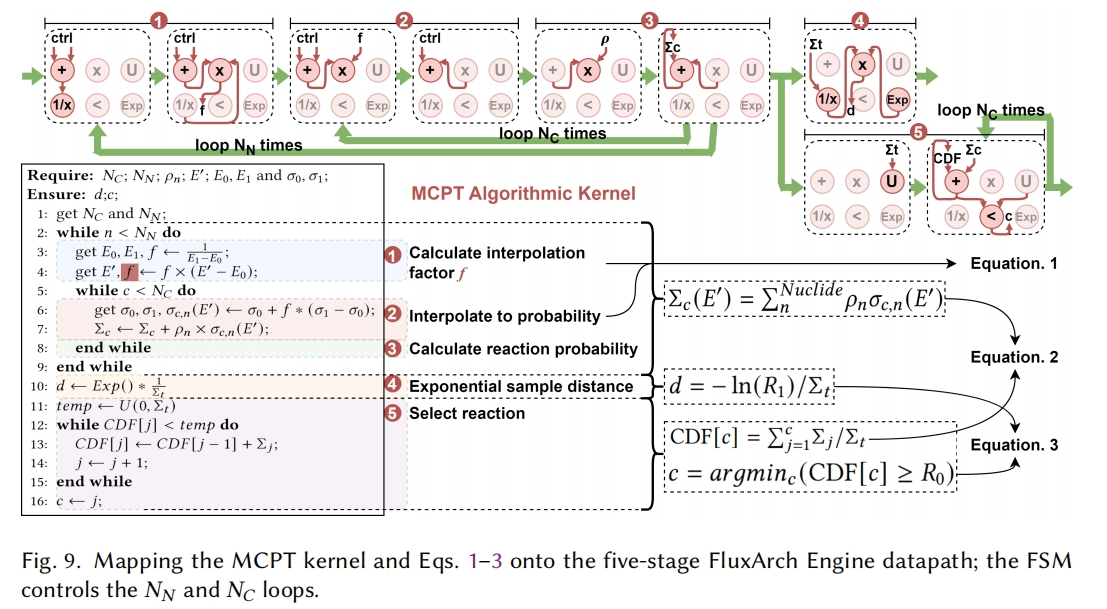
\includegraphics[width=0.9\textwidth]{figures/fig9.png}}
\end{figure}
\end{minipage}\par\medskip

\excerptlabel{Added (Section 4.2, pages 9--10):}\par
\begin{manuscriptexcerpt}
\redsentence{Here, $N_N$ denotes the number of nuclides and $N_C$ the number of reaction channels per nuclide; they determine the outer and inner loop bounds, respectively.}

\redsentence{\textbf{Deterministic Timing Model.}} \redsentence{To meet the timing requirements at the same target clock frequency as the \name\ Core, the RTL operators are partitioned into different numbers of pipeline stages.} \redsentence{Table~2(b) lists the fixed RTL operator latencies using the same symbols as Fig.~9.} \redsentence{Under the computation-only boundary used by the Engine model---excluding launch, stage-transition, \texttt{out\_valid}, and CPU/MMIO input-wait cycles---the five stages take 10 cycles for \redone~($+\to1/x\to\times$, $3+4+3$), 12 cycles for \redtwo~and \redthree~combined~($+\to\times\to+\to\times$, $3+3+3+3$), 7 cycles for \redfour~($1/x\to\times$, $4+3$), and $3+4N_C$ cycles for \redfive~($U\to\{+\to<\}^{N_C}$, $3+N_C(3+1)$).} \redsentence{The resulting latency is
\[
\begin{array}{rl}
L_{\mathrm{Engine}}(N_N,N_C)
&=N_N(10+12N_C)+\max(7,3+4N_C) \\
&=12N_NN_C+10N_N+4N_C+3.
\end{array}
\]} \redsentence{It depends only on the programmed nuclide and reaction-channel counts, not on the numerical operand values.} \redsentence{The gem5 Engine timing directly implements this RTL-derived expression rather than an empirically fitted latency.}
\end{manuscriptexcerpt}



\par\noindent\begin{minipage}{\linewidth}
\revisionlocation{The operator latencies and five-stage timing parameters supporting this derivation are added in \textbf{Table~2(b)}.}

\excerptlabel{Added (Table~2(b), page 10):}\par
% Revised manuscript: Table 2(b)
\begin{figure}[H]
  \centering
  \fbox{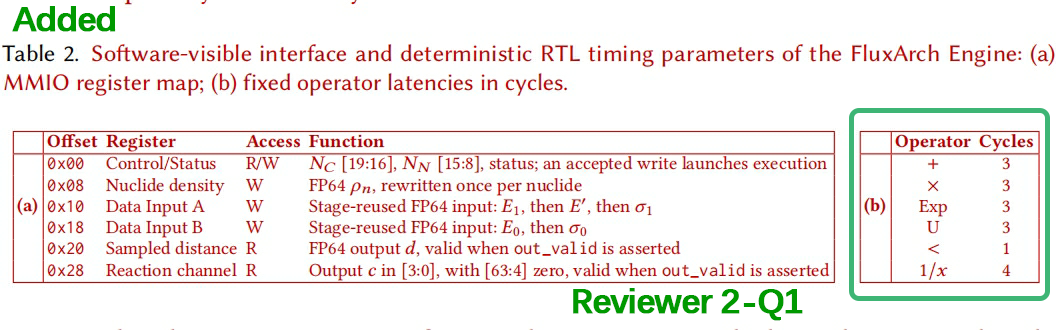
\includegraphics[width=0.9\textwidth]{news/R2-Q1-tab2b.png}}
\end{figure}
\end{minipage}\par\medskip


\revisionlocation{The matched silicon/simulation calibration protocol, errors, and validation scope are described in \textbf{Section 6.1}.}

\excerptlabel{Added (Section 6.1, page 13):}\par
\begin{manuscriptexcerpt}
\redsentence{\textbf{Core Timing Calibration.}} \redsentence{We calibrate the 2-GHz in-order \name\ Core model against a 2-GB KickPi K3B with a 22-nm quad-core RK3562 Cortex-A53~\papercite{kickpi-k3b,rockchip-rk3562}.} \redsentence{The native process is pinned to one 2-GHz core under stable thermal conditions; both platforms use identical source, GCC 13.3, \texttt{-O2 -fno-tree-vectorize}, seed, warm-up, and timed region.} \redsentence{All six checksums match.} \redsentence{Table~3 reports latency and signed error $100(T_{\rm gem5}-T_{\rm K3B})/T_{\rm K3B}$; across the six tests, the mean and maximum absolute percentage errors are 6.7\% and 13.5\%, respectively.} \redsentence{FluxArch's absolute throughput and speedups are obtained directly from the calibrated simulations.}

\redsentence{This silicon comparison calibrates the core and cache/DRAM paths, not the complete 1,024-core hierarchy.} \redsentence{Section~4.2 establishes RTL-to-gem5 Engine timing traceability, and Sections~6.5--6.7 evaluate the modeled full system; we therefore report calibrated simulation evidence, not fabricated-system measurements.}
\end{manuscriptexcerpt}
\begin{excerptreferences}
\paperreference{rockchip-rk3562}
\paperreference{kickpi-k3b}
\end{excerptreferences}

\par\noindent\begin{minipage}{\linewidth}
\revisionlocation{The six RK3562 calibration cases and measured-versus-simulated latencies are added in \textbf{Table~3}.}

\excerptlabel{Added (Table~3, page 13):}\par
% Revised manuscript: Table 3
\begin{figure}[H]
  \centering
  \fbox{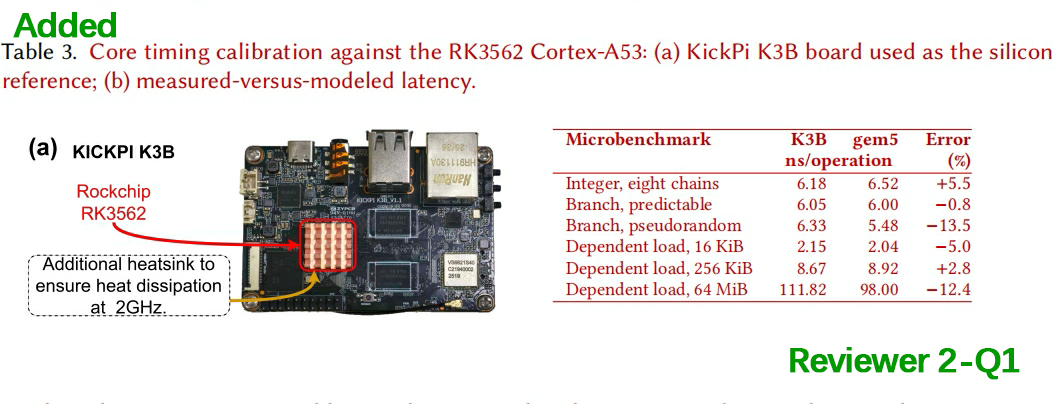
\includegraphics[width=0.9\textwidth]{news/R2-Q1-tab3.png}}
\end{figure}
\end{minipage}\par\medskip


\end{enumerate}

\subsection{Question 2}
\begin{reviewcomment}
Resolve the L2-residency contradiction. Quantify per benchmark whether the replicated database fits in the 4 MB L2 (esp. XSBench); this conflicts with Fig. 3(e) and underpins the speedups.
\end{reviewcomment}
Our performance evaluation does not assume that the benchmark databases reside entirely in L2. The gem5 cache model accounts for finite cache capacity, cache-line replacement, and accesses to the memory hierarchy following L2 misses. The reported throughput therefore reflects capacity-limited caching and the effects of the configured replacement policy, rather than idealized all-hit behavior. For XSBench, the 64.58\% L2 read hit rate and 617.79 bytes of DRAM reads per lookup in Table~6(a) explicitly demonstrate that substantial off-chip accesses remain.

The capacity evidence in Fig.~3(d,e) is consistent with this evaluation. Fig.~3(d) lists a 241~MB complete database and a 62~MB energy-dense working set even for the Small configuration, both exceeding the 4~MB cluster-local L2. These sizes explain the cache-overflow schematic in Fig.~3(e): neither the complete database nor the energy-dense working set can fit in L2. However, capacity overflow does not preclude caching and reusing a subset of lines.

We revised the description of LLC-aware mapping to clarify that the strategy benefits from partial data reuse within each cluster's shared L2 and does not require the entire benchmark database to fit in its 4 MiB capacity. To support this clarification, we added per-workload database size, L2 hit rate, and normalized DRAM traffic. The Quicksilver databases occupy only 0.055--0.318 MiB, whereas the 241-MiB XSBench database is approximately $60.25\times$ the L2 capacity; XSBench therefore cannot reside in L2, although its shared read-only accesses still obtain partial temporal reuse.

\revisionlocation{The full-residency implication is corrected in \textbf{Section 5.2} and \textbf{Figure 3}, which now describes capacity-limited reuse within the shared L2.}

\par\noindent\begin{minipage}{\linewidth}
\excerptlabel{Figure~3 (page 5):}\par
% Manuscript: Figure 3
\begin{figure}[H]
  \centering
  \fbox{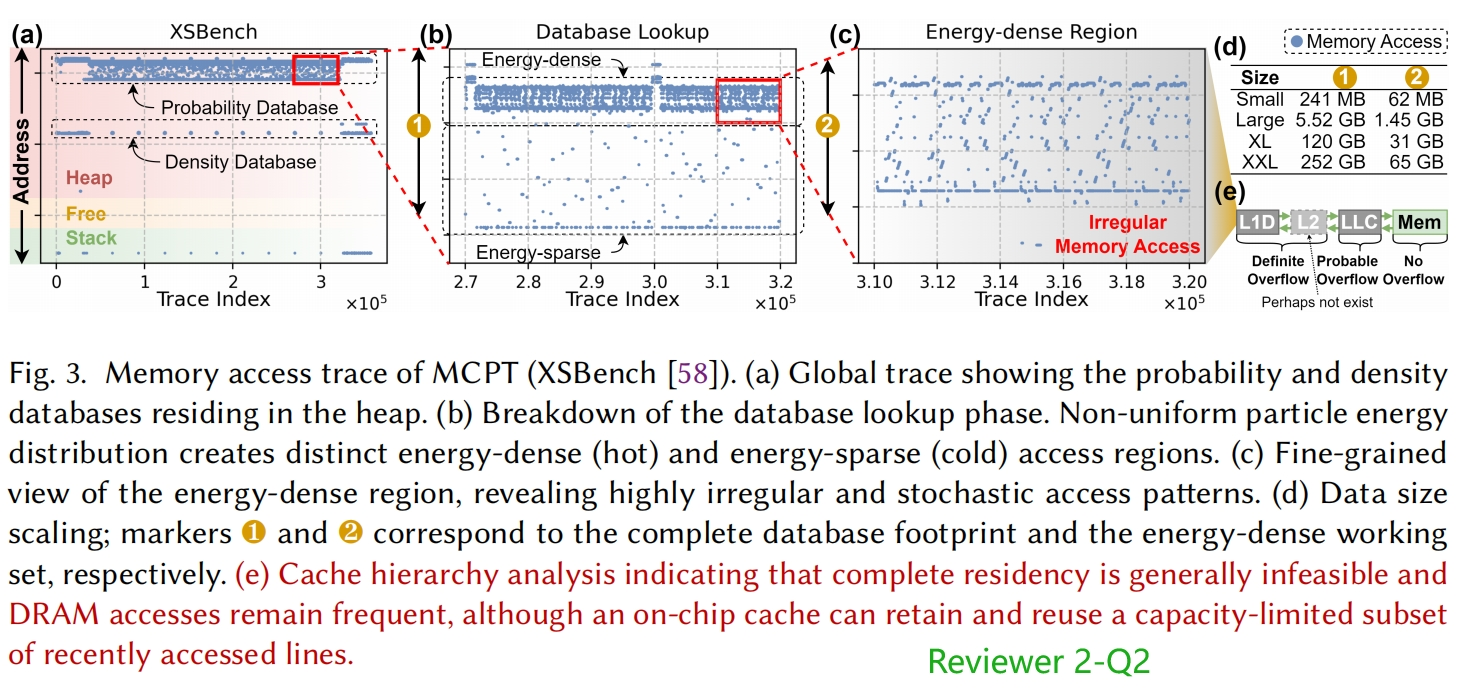
\includegraphics[width=0.9\textwidth]{figures/fig3.png}}
\end{figure}
\end{minipage}\par\medskip

\excerptlabel{Original (Section 5.2, page 12):}\par
\begin{manuscriptexcerpt}
\graysentence{Locality-Optimized Data Replication: The hybrid model treats each process as an isolated memory domain, allowing us to replicate read-only density database and other shared data into local memory.} \graysentence{Provided the dataset fits within the LLC, this converts memory-bound irregular lookups into low-latency L2 cache hits, bypassing the DRAM bottleneck.}
\end{manuscriptexcerpt}


\excerptlabel{Revised (Section 5.2, pages 11--12):}\par
\begin{manuscriptexcerpt}
\redsentence{Shared-Database Reuse within an LLC Domain: Threads belonging to the same MPI process access a common read-mostly physics database.} \redsentence{Binding these threads to cores sharing the cluster-local 4~MB L2 allows a cache line fetched by one thread to be reused by other threads in the process.} \redsentence{This optimization does not require the complete database or working set to reside in L2.} \redsentence{Instead, the shared L2 retains a capacity-limited subset of recently accessed cache lines, reducing rather than eliminating DRAM accesses.} \redsentence{Each process places its database replica in its local NUMA memory domain, avoiding remote-memory accesses when an L2 miss occurs.}
\end{manuscriptexcerpt}

\revisionlocation{The workload-dependent L2 residency and DRAM traffic are analyzed in \textbf{Section 6.5}.}

\excerptlabel{Added (Section 6.5, pages 17--18):}\par
\begin{manuscriptexcerpt}
\redsentence{Table~6(a) clarifies that the affinity strategy does not rely on universal database residency in the 4~MB cluster-local L2.} \redsentence{The databases of CORAL2-P1, CORAL2-P2, CTS2 and Homogeneous occupy only 0.055--0.318~MiB per process and achieve 91.98\%--95.81\% L2 read hit rates.} \redsentence{In contrast, the 241~MiB XSBench database is approximately 60$\times$ the L2 capacity.} \redsentence{Nevertheless, its 64.58\% L2 read hit rate shows that the cache retains a useful capacity-limited subset, while the remaining misses generate 617.79 bytes of DRAM reads per lookup.} \redsentence{For Quicksilver, DRAM traffic is normalized per transported segment; for XSBench, it is normalized per cross-section lookup.} \redsentence{These measurements are consistent with the intended mechanism: the shared L2 captures partial reuse but neither requires complete working-set residency nor eliminates DRAM traffic.}
\end{manuscriptexcerpt}

\par\noindent\begin{minipage}{\linewidth}
\revisionlocation{The database sizes, L2 hit rates, and normalized DRAM traffic are added in \textbf{Table~6(a)}.}

\excerptlabel{Added (Table~6(a), page 18):}\par
% Revised manuscript: Table 6(a)
\begin{figure}[H]
  \centering
  \fbox{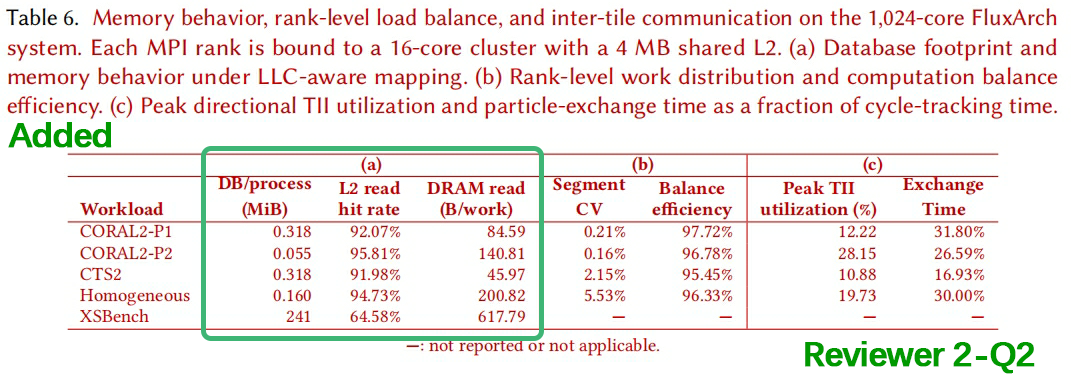
\includegraphics[width=0.9\textwidth]{news/R2-Q2-tab6a.png}}
\end{figure}
\end{minipage}\par\medskip

\subsection{Question 3}

\begin{reviewcomment}
Report DRAM-inclusive energy, or justify why excluding off-chip DRAM does not bias a memory-bound workload.
\end{reviewcomment}

We agree that excluding DRAM would bias the system-level energy comparison for these memory-intensive workloads. We changed the evaluation to include co-packaged DDR4/HBM through device telemetry and off-package DDR5 through the same traffic-based DRAMPower methodology, and we vary the modeled DDR5 component over a $0.5\times$--$2\times$ range to assess sensitivity. The conservative process-scaled geometric-mean DRAM-inclusive energy-efficiency advantage remains 1.77$\times$ over H100 and 6.65$\times$ over Intel.

We now explain the choice of the $0.5\times$--$2\times$ range in \textbf{Section 6.1}. Ghose et al.~\papercite{ghose2018vampire} measured DDR3L read currents averaging 54.1\% below datasheet values for one vendor and data-pattern-dependent read-power differences of up to 91.6\%. Shi et al.~\papercite{shi2025drampower} report that DDR4 calibration reduced DRAMPower energy estimates by roughly half for most evaluated SPEC2006 workloads. These results motivate testing sizable modeling discrepancies, but do not establish an error bound for our DDR5 configuration. We therefore select reciprocal factors of 0.5 and 2 to test both overestimation and underestimation, with package power fixed; the range is a sensitivity-analysis choice, not a statistical confidence interval.

For process-scaled energy-efficiency bounds, we independently vary only the scaled FluxArch package power by $\pm30\%$ and each modeled off-package DRAM component over $0.5\times$--$2\times$, while keeping throughput and measured baseline package power fixed. We recompute the performance/W ratio at every endpoint combination and report its minimum and maximum; external DRAM power is not subject to process-node scaling or its 30\% margin.

\begin{excerptreferences}
\paperreference{ghose2018vampire}
\paperreference{shi2025drampower}
\end{excerptreferences}

\revisionlocation{The common DRAM-power accounting model and sensitivity bounds are specified in \textbf{Section 6.1}.

The DRAM-inclusive energy-efficiency results and conservative lower bounds are updated in \textbf{Section 6.2}.}

\excerptlabel{Original (Section 6.2, pages 14--15):}\par
\begin{manuscriptexcerpt}
\graysentence{\textbf{Iso-Process Energy Efficiency}.} \graysentence{As shown in Fig.~13(b), the energy efficiency advantage is even more pronounced.} \graysentence{By comparing projected iso-process nodes, we isolate the architectural contributions.} \graysentence{According to Section. 6.1, the power projection error is 30\%.} \graysentence{Therefore, we incorporate this margin into our energy efficiency evaluation, which is represented as error bars in our results.} \graysentence{Without the workload orchestration, the energy efficiency of \name, mainstream server CPUs and high-end GPUs is at odds with each other.} \graysentence{With the orchestration enabled, optimizing data locality and minimizing cross-tile traffic, \name\ demonstrates a superior geometric mean energy efficiency improvement from \textbf{3.98}$\boldsymbol{\times}$ (vs. \ft, 5.69$\times$ discounted by 30\%) to \textbf{9.84}$\boldsymbol{\times}$ (vs. \intel, 14.06$\times$ discounted by 30\%) even accounting for the potential projection error of pessimistic assumption.} \graysentence{We also report the energy efficiency of the raw, unscaled data based on the 22 nm technology node.} \graysentence{Even in this case, \name\ still achieves an energy efficiency improvement of 1.17$\times$ (vs. \hopper) to 4.59$\times$ (vs. \intel).}
\end{manuscriptexcerpt}

\excerptlabel{Revised (Section 6.2, pages 15--16):}\par
\begin{manuscriptexcerpt}
\redsentence{\textbf{DRAM-Inclusive Energy Efficiency.}} \redsentence{Fig.~13(c,d) reports DRAM-inclusive power and energy efficiency under the sensitivity bounds defined in Section~6.1.} \redsentence{Process-scaled results separate architectural effects from process scaling while accounting consistently for external memory.}

\redsentence{In the process-scaled comparison, \name\ improves geometric-mean DRAM-inclusive efficiency by \textbf{2.85}$\boldsymbol{\times}$ over \hopper\ to \textbf{10.58}$\boldsymbol{\times}$ over \intel.}

\redsentence{The sensitivity analysis preserves the process-scaled conclusion: across the combined DRAM and technology-scaling bounds, the geometric-mean improvement with orchestration remains 1.77$\times$ over \hopper\ and 6.65$\times$ over \intel\ at the conservative lower bound.}
\end{manuscriptexcerpt}

\par\noindent\begin{minipage}{\linewidth}
\revisionlocation{The DRAM-inclusive power breakdown and energy-efficiency results are plotted in revised \textbf{Figure~13(c,d)}. Panel (c) is newly added; panel (d) revises the original energy-efficiency plot.}

\excerptlabel{Original (Figure~13, page 15):}\par
% Original manuscript: Figure 13
\begin{figure}[H]
  \centering
  \fbox{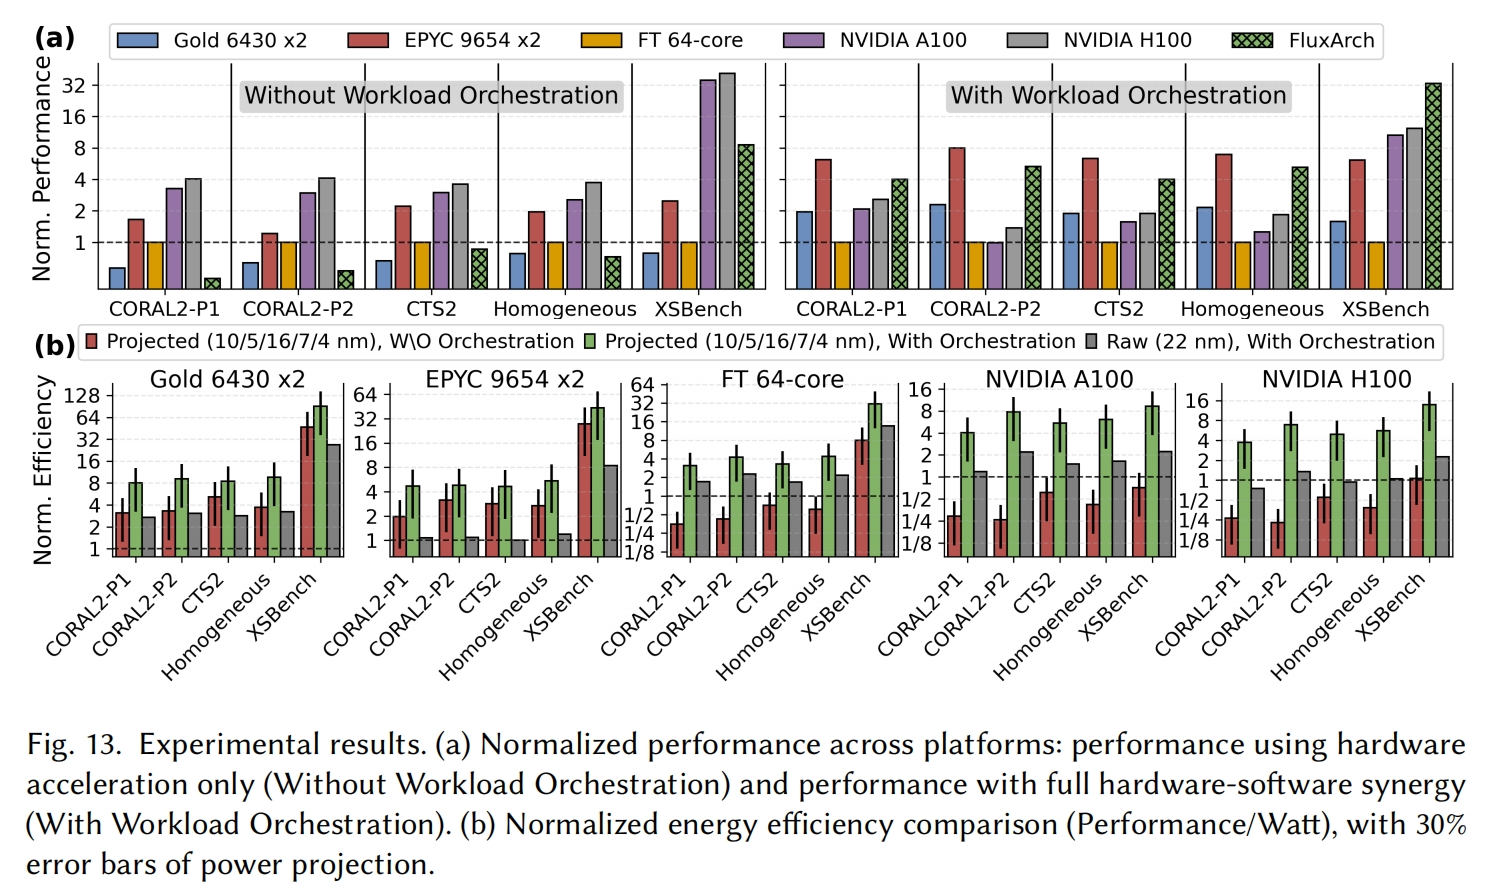
\includegraphics[width=0.9\textwidth]{figures/O-fig13.png}}
\end{figure}
\end{minipage}\par\medskip

\par\noindent\begin{minipage}{\linewidth}
\excerptlabel{Revised (Figure~13, page 16):}\par
% Revised manuscript: Figure 13
\begin{figure}[H]
  \centering
  \fbox{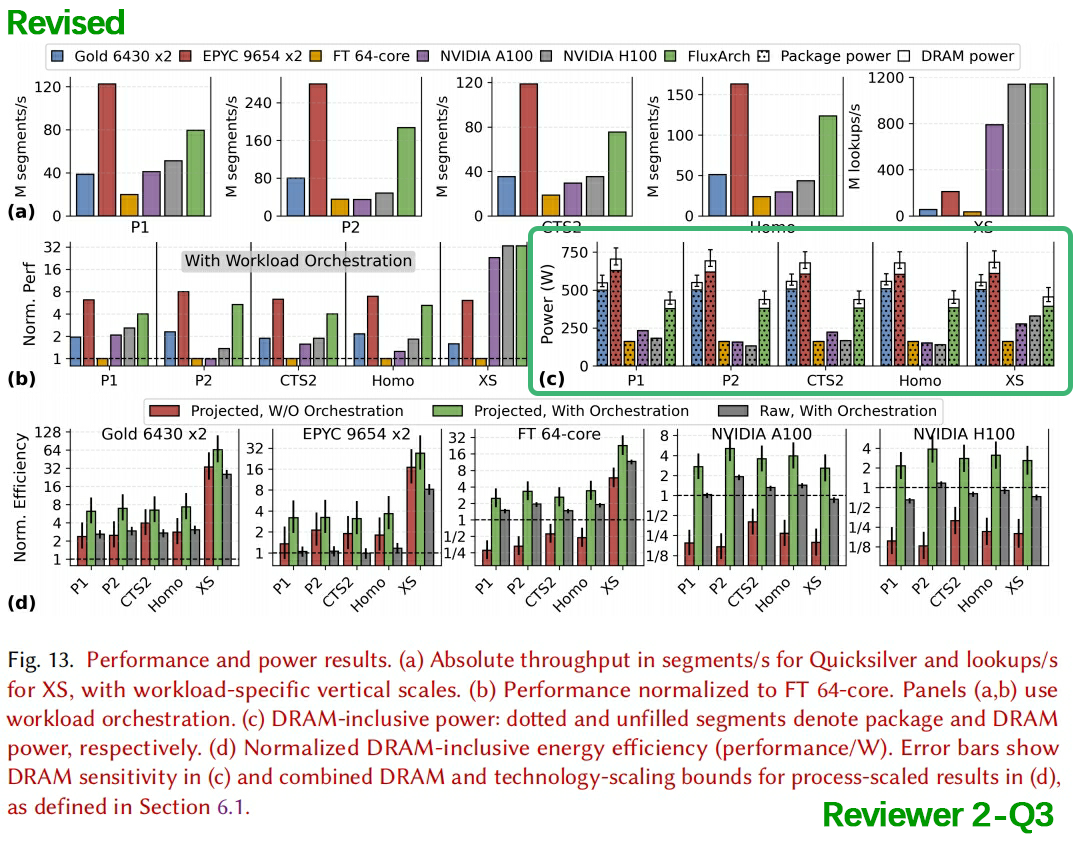
\includegraphics[width=0.9\textwidth]{news/R2-Q3-fig13.png}}
\end{figure}
\end{minipage}\par\medskip

\subsection{Question 4}
\begin{reviewcomment}
Fix inconsistencies and add absolutes. Reconcile the conflicting engine-area and energy figures, report absolute throughput (histories/sec), and do a language pass.
\end{reviewcomment}
We reconciled the Engine-area and energy-efficiency figures, added absolute throughput, and revised the language.

\begin{enumerate}[label=(\arabic*)]
\setlength{\emergencystretch}{1em}
\item \textbf{Engine-area consistency.} The correct synthesized Engine area is 0.270~mm$^2$, compared with 0.763~mm$^2$ for the standard FPU. We corrected the inconsistent value and percentage throughout the manuscript. The consistent result is that the Engine occupies 35.4\% of the FPU area, corresponding to a 64.6\% reduction.

\revisionlocation{The Engine-area value and its comparison with the standard FPU are corrected in \textbf{Section 3.3}.}

\excerptlabel{Original (Section 3.3, page 7):}\par
\begin{manuscriptexcerpt}
\graysentence{To evaluate the area efficiency of architectural specialization, we synthesized both a standard full-functional FPU and our engine using open-source RTL at a 22 nm technology node (as detailed in Section 6.3).} \graysentence{By eliminating the extensive logic required for full FP32/FP64 precision and stripping away general-purpose scheduling, our dedicated engine occupies only 0.251~mm$^2$---a 67\% reduction in footprint compared to a standard FPU (0.763~mm$^2$).} \graysentence{This specialized FP64-only design maximizes computational density per unit area, directly addressing the low arithmetic intensity of general-purpose cores while providing the throughput necessary for large-scale MCPT simulations.}
\end{manuscriptexcerpt}

\excerptlabel{Revised (Section 3.3, page 6):}\par
\begin{manuscriptexcerpt}
\graysentence{To evaluate the area efficiency of architectural specialization, we synthesized both a standard full-functional FPU and our engine using open-source RTL~\papercite{hardfloat} at a 22 nm technology node (as detailed in Section 6.3).} \redsentence{By eliminating the extensive logic required for full FP32/FP64 precision and stripping away general-purpose scheduling, our dedicated engine occupies 0.270~mm$^2$---a 64.6\% reduction in footprint compared with a standard FPU (0.763~mm$^2$).} \graysentence{This specialized FP64-only design maximizes computational density per unit area, directly addressing the low arithmetic intensity of general-purpose cores while providing the throughput necessary for large-scale MCPT simulations.}
\end{manuscriptexcerpt}
\begin{excerptreferences}
\paperreference{hardfloat}
\end{excerptreferences}

\revisionlocation{The area analysis is corrected in \textbf{Section 6.3} to use the same Engine area and reduction percentage.}

\excerptlabel{Original (Section 6.3, page 15):}\par
\begin{manuscriptexcerpt}
\graysentence{The system hierarchy is optimized for high computational density (Fig.~14(c)), with Compute Tiles dominating the design (97\% of total area) and compute cores accounting for approximately 70\% of the entire system's area.} \graysentence{The \name\ Engine, shown in Fig.~14(b), is remarkably area-efficient, occupying only one-third of the footprint of a standard FPU.} \graysentence{This specialization for MCPT achieves higher throughput per mm$^2$ than general-purpose units.} \graysentence{A detailed floorplan of the Engine (Fig.~14(a)) reveals a total area of 0.27~mm$^2$, where FP64 functional units occupy over 97\% of the engine's area.} \graysentence{This extreme functional density is achieved by stripping away single-precision support and complex control logic, dedicating nearly all silicon to the primary computational bottlenecks of MCPT.}
\end{manuscriptexcerpt}

\excerptlabel{Revised (Section 6.3, page 17):}\par
\begin{manuscriptexcerpt}
\graysentence{The system hierarchy is optimized for high computational density (Fig.~14(c)), with Compute Tiles dominating the design (97\% of total area) and compute cores accounting for approximately 70\% of the entire system's area.} \redsentence{The \name\ Engine, shown in Fig.~14(b), is remarkably area-efficient, occupying 0.270~mm$^2$, or 35.4\% of the 0.763~mm$^2$ standard-FPU footprint.} \graysentence{This specialization for MCPT achieves higher throughput per mm$^2$ than general-purpose units.} \redsentence{A detailed floorplan of the Engine (Fig.~14(a)) shows that FP64 functional units occupy over 97\% of the engine area.} \graysentence{This extreme functional density is achieved by stripping away single-precision support and complex control logic, dedicating nearly all silicon to the primary computational bottlenecks of MCPT.}
\end{manuscriptexcerpt}


\item \textbf{Energy-efficiency consistency.} The original manuscript mixed nominal energy-efficiency improvements (5.69$\times$--14.06$\times$ in the Introduction) with conservative values after a 30\% discount (3.98$\times$--9.84$\times$ in Section 6.2 and the Conclusion), without consistently distinguishing the two. We have unified the reporting convention for the updated evaluation: the Abstract, Introduction, Section 6.2, and Conclusion now report nominal process-scaled, DRAM-inclusive energy-efficiency results, with geometric-mean improvements of 2.85$\times$ over H100 to 10.58$\times$ over Intel (the Abstract reports the maximum geometric-mean improvement across the evaluated baselines). Section 6.2 separately identifies 1.77$\times$ over H100 and 6.65$\times$ over Intel as conservative lower bounds under the combined DRAM and technology-scaling uncertainties. These updated results incorporate the revised DRAM accounting and GPU baseline described in our other responses; they are not a relabeling of the original measurements.

\revisionlocation{The evaluation contribution in \textbf{Section 1} is revised to report the updated nominal process-scaled, DRAM-inclusive energy-efficiency range.}

\excerptlabel{Original (Section 1, page 3):}\par
\begin{manuscriptexcerpt}
\graysentence{We evaluate \name\ via full-system modeling across industrial-grade benchmarks.} \graysentence{Experimental results demonstrate that \name\ achieves a geometric mean speedup of $1.02\times$ to $6.83\times$ and energy efficiency improvements of $5.69\times$ to $14.06\times$ compared to high-performance server-class CPUs and GPUs.}
\end{manuscriptexcerpt}

\excerptlabel{Revised (Section 1, page 2):}\par
\begin{manuscriptexcerpt}
\graysentence{We evaluate \name\ via full-system modeling across industrial-grade benchmarks.} \graysentence{The evaluation combines package power with measured or traffic-modeled memory power, depending on whether memory is co-packaged or off-package, and uses a sorting-enabled XSBench implementation as the GPU baseline.} \redsentence{Experimental results demonstrate that \name\ achieves a geometric mean speedup of $1.02\times$ to $6.83\times$ and process-scaled DRAM-inclusive energy-efficiency improvements of $2.85\times$ to $10.58\times$ compared to high-performance server-class CPUs and GPUs.}
\end{manuscriptexcerpt}

\revisionlocation{The result summary in \textbf{Section 9} is revised to replace the original discounted energy-efficiency range with the updated nominal process-scaled, DRAM-inclusive range, consistent with Section 1.}

\excerptlabel{Original (Section 9, page 20):}\par
\begin{manuscriptexcerpt}
\graysentence{By co-optimizing hardware topology and spatial decomposition, \name\ overcomes irregular memory access limitations and delivers geometric mean speedups of up to 1.02$\times$-6.83$\times$ and energy efficiency improvements of up to 3.98$\times$-9.84$\times$ over traditional processors.}
\end{manuscriptexcerpt}

\excerptlabel{Revised (Section 9, page 23):}\par
\begin{manuscriptexcerpt}
\graysentence{By co-optimizing hardware topology and spatial decomposition, \name\ overcomes irregular memory access limitations.} \graysentence{Using a sorting-enabled XSBench implementation for the GPU comparison, \name\ delivers geometric mean speedups of 1.02$\times$--6.83$\times$ over traditional processors.} \redsentence{It also delivers process-scaled DRAM-inclusive energy-efficiency improvements of 2.85$\times$--10.58$\times$.}
\end{manuscriptexcerpt}

\revisionlocation{The nominal results and conservative lower bounds are distinguished explicitly in \textbf{Section 6.2}.}

\excerptlabel{Revised (Section 6.2, page 16):}\par
\begin{manuscriptexcerpt}
\redsentence{In the process-scaled comparison, \name\ improves geometric-mean DRAM-inclusive efficiency by \textbf{2.85}$\boldsymbol{\times}$ over \hopper\ to \textbf{10.58}$\boldsymbol{\times}$ over \intel.} \redsentence{The sensitivity analysis preserves the process-scaled conclusion: across the combined DRAM and technology-scaling bounds, the geometric-mean improvement with orchestration remains 1.77$\times$ over \hopper\ and 6.65$\times$ over \intel\ at the conservative lower bound.}
\end{manuscriptexcerpt}

\item \textbf{Absolute throughput.} The original normalized plot did not expose the absolute performance represented by each workload-specific metric. We revised the evaluation to report absolute throughput alongside the normalized comparison, using segments/s for CORAL2-P1, CORAL2-P2, CTS2 and Homogeneous and lookups/s for XSBench. We report the benchmark-specific equivalents of histories/s: segments/s for Quicksilver and lookups/s for XSBench. \name\ achieves 79.33, 186.70, 75.33, and 123.50 million segments/s for P1, P2, CTS2, and Homogeneous, respectively, and 1.143 billion XSBench lookups/s.

\revisionlocation{The absolute throughput values and workload-specific units are reported in \textbf{Section 6.2}.}

\excerptlabel{Revised (Section 6.2, page 15):}\par
\begin{manuscriptexcerpt}
\graysentence{\textbf{Performance Impact}.} \redsentence{Fig.~13(a,b) reports absolute throughput and values normalized to \ft.} \redsentence{\name\ achieves 79.33, 186.70, 75.33, and 123.50 million segments/s for P1, P2, CTS2, and Homo, respectively, and 1.143 billion XS lookups/s, yielding geometric-mean speedups from \textbf{1.02}$\boldsymbol{\times}$ over \amd\ to \textbf{6.83}$\boldsymbol{\times}$ over \ft.}
\end{manuscriptexcerpt}

\par\noindent\begin{minipage}{\linewidth}
\revisionlocation{\textbf{Figure~13(a)} adds absolute throughput, while \textbf{Figure~13(b)} revises the original normalized-performance plot.}

\excerptlabel{Original (Figure~13, page 15):}\par
% Original manuscript: Figure 13
\begin{figure}[H]
  \centering
  \fbox{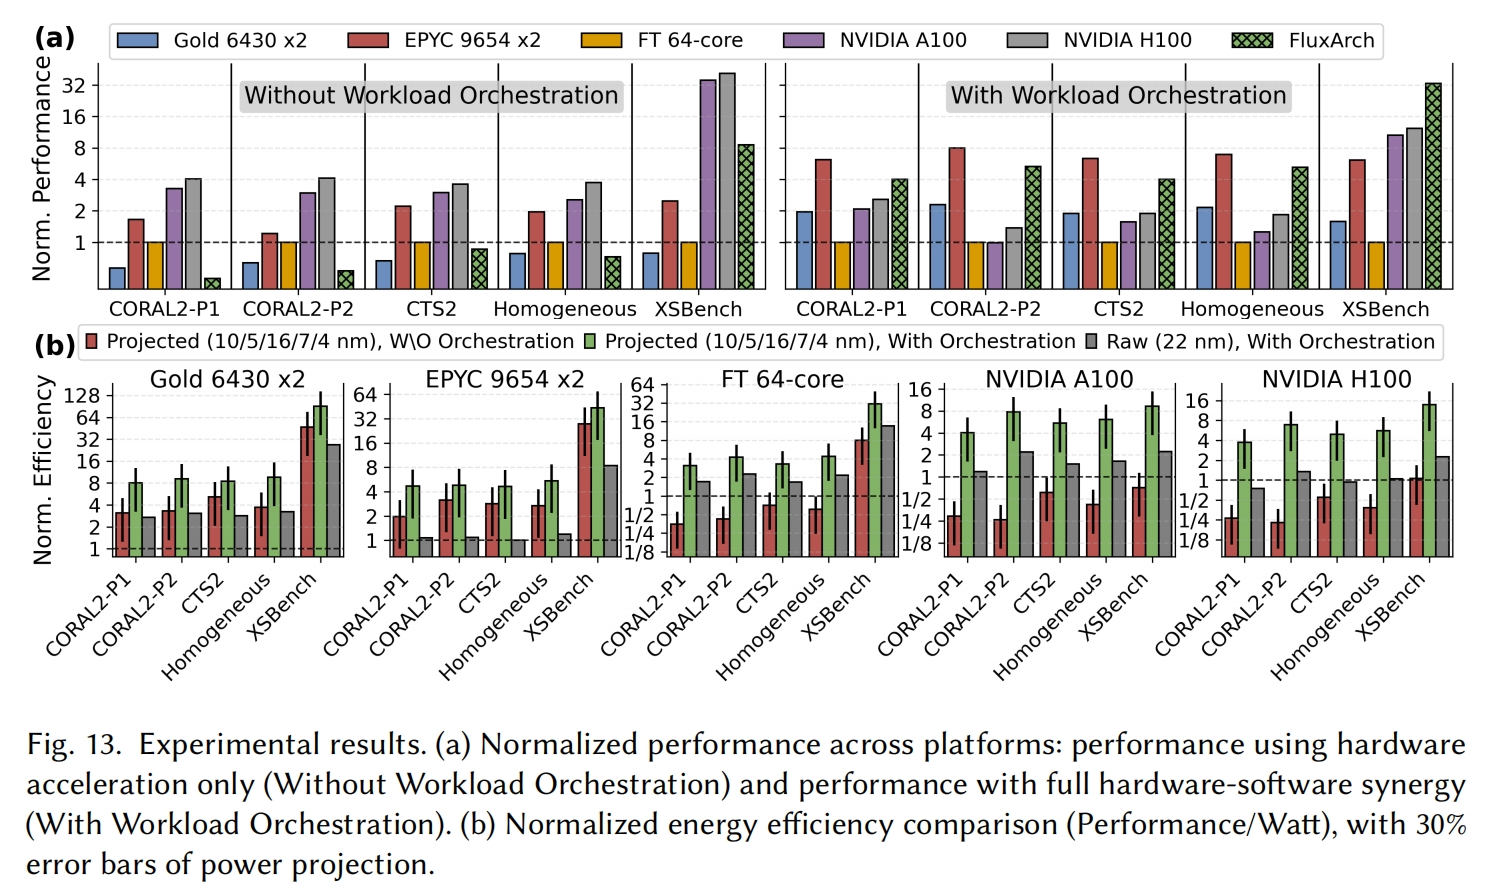
\includegraphics[width=0.9\textwidth]{figures/O-fig13.png}}
\end{figure}
\end{minipage}\par\medskip

\par\noindent\begin{minipage}{\linewidth}
\excerptlabel{Revised (Figure~13, page 16):}\par
% Revised manuscript: Figure 13
\begin{figure}[H]
  \centering
  \fbox{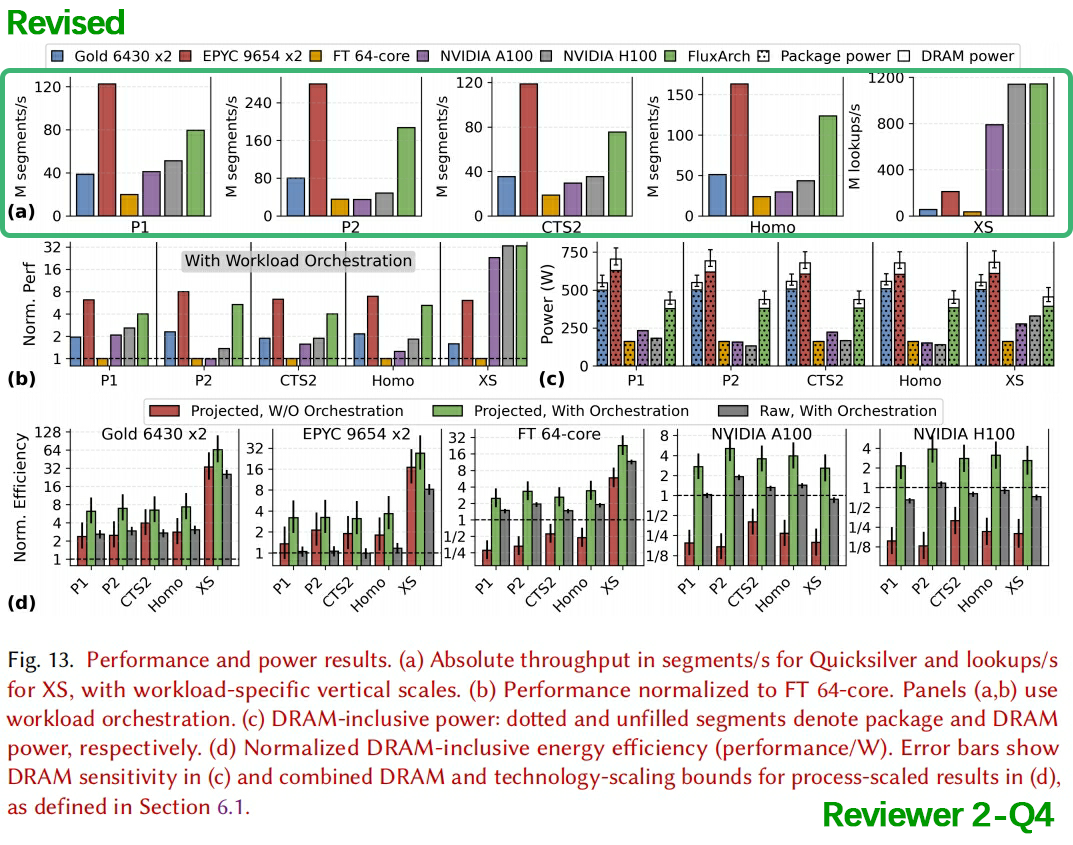
\includegraphics[width=0.9\textwidth]{news/R2-Q4-fig13.png}}
\end{figure}
\end{minipage}\par\medskip

\item \textbf{Language revision.} We carefully reviewed the language throughout the manuscript. Specifically, we corrected spelling and typographical errors, fixed grammatical issues, revised awkward sentence structures, and rephrased passages to improve clarity, fluency, and readability.

For example, in the caption of \textbf{Figure~19} in \textbf{Section 6.7}, we condensed the original three-sentence description into: ``Inter-core latency; right-side triangles denote averages, and steps mark CCD, cluster, tile, and socket boundaries.'' This replaces verbose wording such as ``The latency curve exhibits a step-like profile reflecting architectural hierarchy boundaries'' with the more direct ``steps mark CCD, cluster, tile, and socket boundaries,'' while retaining the explanation of the plotted markers and hierarchy boundaries.

\par\noindent\begin{minipage}{\linewidth}
\excerptlabel{Original (Figure~18, page 18):}\par
% Original manuscript: Figure 18
\begin{figure}[H]
  \centering
  \fbox{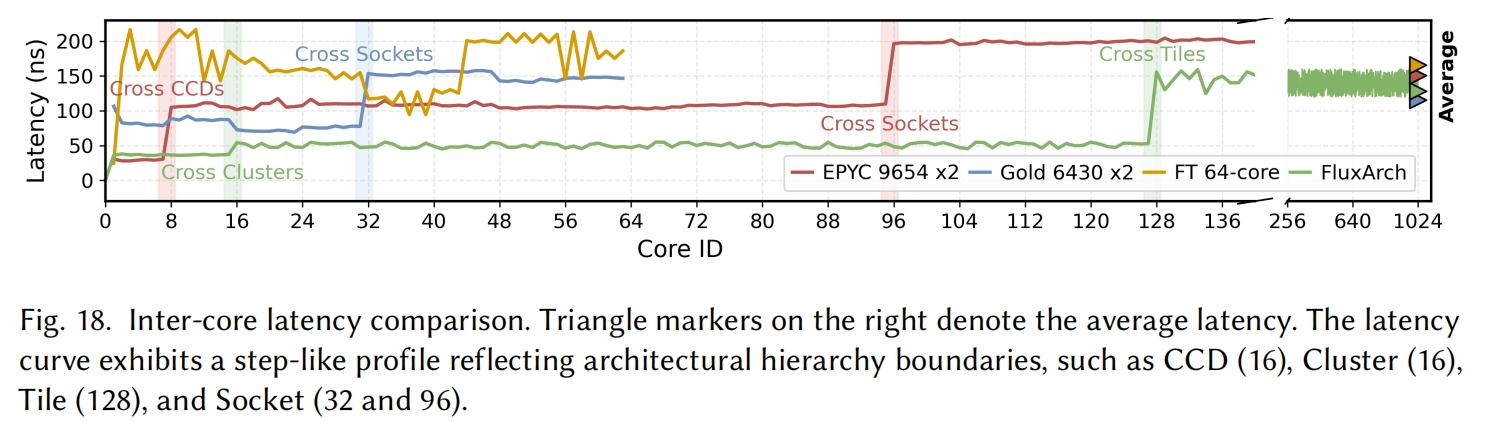
\includegraphics[width=0.9\textwidth]{figures/O-fig18.png}}
\end{figure}
\end{minipage}\par\medskip

\par\noindent\begin{minipage}{\linewidth}
\excerptlabel{Revised (Figure~19, page 21):}\par
% Revised manuscript: Figure 19
\begin{figure}[H]
  \centering
  \fbox{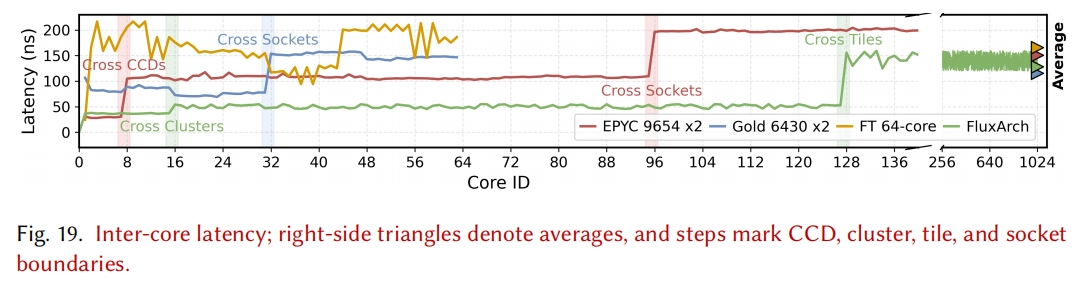
\includegraphics[width=0.9\textwidth]{news/R2-Q4-fig19.png}}
\end{figure}
\end{minipage}\par\medskip

\end{enumerate}

\subsection{Question 5}
\begin{reviewcomment}
Acknowledged but not quantified: DRAM-inclusive energy (Sec. 6.1 excludes it); whether the working set fits in 4 MB L2 --- which contradicts Fig. 3(e); load imbalance on non-uniform inputs (Sec. 7). Absent: inter-tile MPI transport and Death-Respawn cost; the MMIO programming/porting interface; absolute throughput; model validation against silicon.
\end{reviewcomment}
We sincerely thank you for your helpful and constructive suggestion. Because this comment collects eight distinct issues, we address them separately.
\begin{enumerate}[label=(\arabic*)]
\setlength{\emergencystretch}{1em}
\item \textbf{DRAM-inclusive energy.} The energy comparison now includes main-memory power rather than using an on-chip-only boundary. We added consistent accounting for co-packaged memory and off-package DDR5 plus a $0.5\times$--$2\times$ sensitivity analysis. The conservative process-scaled advantage remains above unity.

\revisionlocation{The memory-power accounting boundary and DRAM sensitivity analysis are clarified in \textbf{Section 6.1}.}

\excerptlabel{Revised (Section 6.1, page 14):}\par
\begin{manuscriptexcerpt}
\redsentence{We report DRAM-inclusive system power and energy.} \redsentence{Package power includes cores, caches, NoCs, and integrated memory controllers; for \ft, \ampare, and \hopper, the main memory is co-packaged (DDR4 or HBM) and is consequently covered by platform-level package/device telemetry.} \redsentence{In contrast, the DDR5 DIMMs of \intel\ and \amd, and the DDR5 channels assumed for \name, are physically off-package and are not covered by package-power readings.} \redsentence{We therefore add a separately modeled DRAM component to these platforms, avoiding asymmetric accounting that would include HBM/DDR4 power for the co-packaged-memory platforms but omit DDR5 power for the other platforms.}
\end{manuscriptexcerpt}

\par\noindent\begin{minipage}{\linewidth}
\revisionlocation{The resulting energy-efficiency comparison is updated in \textbf{Section 6.2}.

The DRAM-inclusive power and energy-efficiency plots are updated in \textbf{Figure~13(c,d)}. Panel (c) is newly added; panel (d) revises the original energy-efficiency plot.}

\excerptlabel{Revised (Figure~13, page 16):}\par
% Revised manuscript: Figure 13
\begin{figure}[H]
  \centering
  \fbox{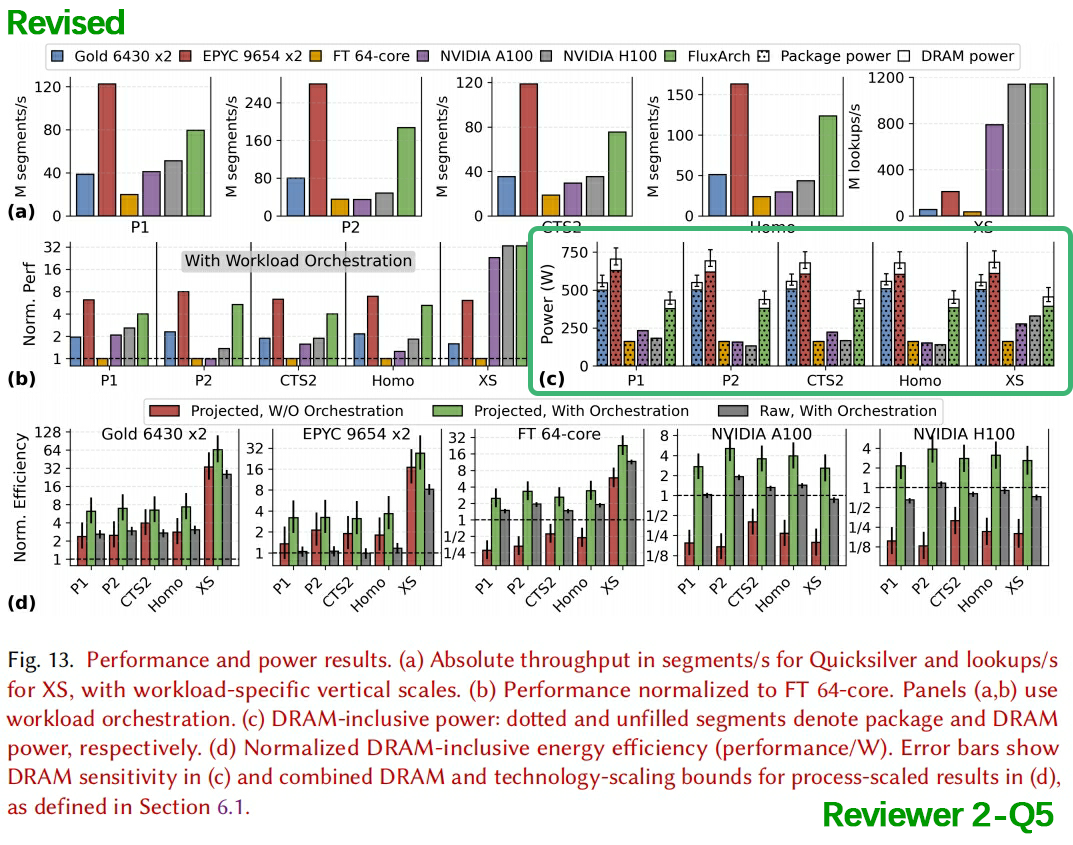
\includegraphics[width=0.9\textwidth]{news/R2-Q5-fig13.png}}
\end{figure}
\end{minipage}\par\medskip

\item \textbf{L2 working-set residency.} Our affinity mechanism provides partial shared-L2 reuse rather than universal full-working-set residency. We corrected the claim and added database-capacity and memory-traffic measurements. The 241-MiB XSBench database is about $60.25\times$ larger than the 4-MiB L2, confirming that its benefit cannot be attributed to complete residency.

\revisionlocation{The affinity mechanism is clarified in \textbf{Section 5.2} as partial shared-L2 reuse rather than full database residency.}

\excerptlabel{Revised (Section 5.2, pages 11--12):}\par
\begin{manuscriptexcerpt}
\redsentence{Shared-Database Reuse within an LLC Domain: Threads belonging to the same MPI process access a common read-mostly physics database.} \redsentence{Binding these threads to cores sharing the cluster-local 4~MB L2 allows a cache line fetched by one thread to be reused by other threads in the process.} \redsentence{This optimization does not require the complete database or working set to reside in L2.} \redsentence{Instead, the shared L2 retains a capacity-limited subset of recently accessed cache lines, reducing rather than eliminating DRAM accesses.} \redsentence{Each process places its database replica in its local NUMA memory domain, avoiding remote-memory accesses when an L2 miss occurs.}
\end{manuscriptexcerpt}

\par\noindent\begin{minipage}{\linewidth}
\revisionlocation{The memory-behavior analysis is added in \textbf{Section 6.5}.

The supporting database-capacity, L2-hit-rate, and DRAM-traffic measurements are added in \textbf{Table~6(a)}.}

\excerptlabel{Added (Table~6(a), page 18):}\par
% Revised manuscript: Table 6(a)
\begin{figure}[H]
  \centering
  \fbox{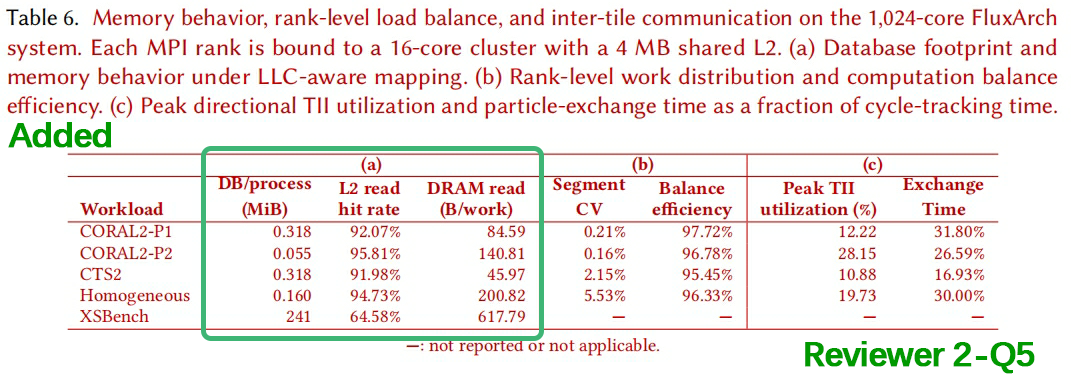
\includegraphics[width=0.9\textwidth]{news/R2-Q5-tab6a.png}}
\end{figure}
\end{minipage}\par\medskip

\item \textbf{Load imbalance.} Static spatial decomposition can create unequal stochastic work, so we added measurements across all 64 cluster-bound MPI ranks. Kernel-time CV is 1.17\%--2.01\%, balance efficiency is 95.45\%--97.72\%, and the estimated computation-side tail loss is at most 4.55\% for the evaluated inputs. These results indicate that static affinity and spatial decomposition maintain balanced computation across clusters for the evaluated workloads at 1,024 cores, with limited computation-side loss from load imbalance. More extreme inputs remain a limitation.

\revisionlocation{The rank-level load-balance evaluation and estimated computation-side tail loss are added in \textbf{Section 6.5}.}

\excerptlabel{Added (Section 6.5, pages 18--19):}\par
\begin{manuscriptexcerpt}
\redsentence{\textbf{Load Balance}.} \redsentence{Table~6(b) quantifies the concern that static affinity and spatial decomposition may assign unequal work to clusters.} \redsentence{We record completed segments and accumulated tracking-kernel time separately for all 64 ranks.} \redsentence{Segment-count CV ranges from 0.16\% to 5.53\%; because stochastic segments can follow different paths and incur different costs, count variation does not translate proportionally into execution-time variation.} \redsentence{Kernel-time CV remains 1.17\%--2.01\%.} \redsentence{We define balance efficiency as the mean rank-level kernel time divided by the maximum rank-level kernel time, since the slowest rank determines the computation tail.} \redsentence{The resulting efficiency is 95.45\%--97.72\%, corresponding to an estimated computation-side tail loss of at most 4.55\%.} \redsentence{These results indicate that static affinity and spatial decomposition maintain balanced computation across clusters for the evaluated workloads at 1,024 cores, with limited computation-side loss from load imbalance.}
\end{manuscriptexcerpt}

\par\noindent\begin{minipage}{\linewidth}
\revisionlocation{The segment-count variation and balance efficiency are reported in \textbf{Table~6(b)}.}

\excerptlabel{Added (Table~6(b), page 18):}\par
% Revised manuscript: Table 6(b)
\begin{figure}[H]
  \centering
  \fbox{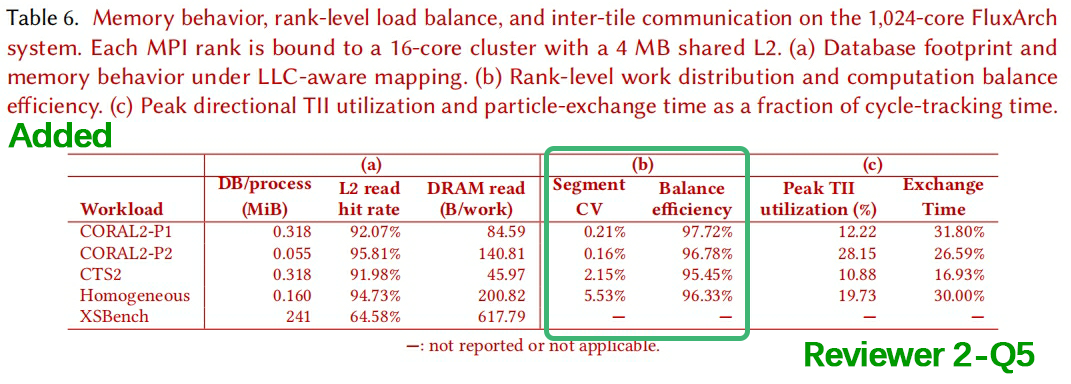
\includegraphics[width=0.9\textwidth]{news/R2-Q5-tab6b.png}}
\end{figure}
\end{minipage}\par\medskip

\item \textbf{Inter-tile MPI transport.} Inter-tile MPI transport is explicitly modeled rather than implemented as zero-cost functional communication. We added the complete path through the guest network stack, IGbE endpoints, and \texttt{DistEtherLink} TIIs and measured traffic at every interface. The busiest direction uses 10.88\%--28.15\% of the modeled 1-Gb/s capacity, with only 0.50\%--2.42\% traffic CV across TIIs.

\revisionlocation{The guest-network, IGbE, and TII transport path is specified in \textbf{Section 6.1}.}

\excerptlabel{Added (Section 6.1, page 13):}\par
\begin{manuscriptexcerpt}
\redsentence{\textbf{Inter-Tile Communication Modeling}.} \redsentence{The eight Compute Tiles are connected to the Switch Tile through eight bidirectional Tile Interconnection Interfaces (TIIs).} \redsentence{In distributed full-system gem5, each TII is modeled using a \texttt{DistEtherLink} and an IGbE endpoint, with the directional 1-Gb/s capacity in Table~1 and the modeled inter-tile latency.} \redsentence{MPI messages traverse the guest network stack and these modeled links and are therefore subject to software protocol processing, packetization, link serialization, and inter-tile latency rather than zero-cost functional communication.} \redsentence{We use the Ethernet-device counters to measure transmitted bytes and directional utilization at every TII.} \redsentence{Quicksilver's cycle-tracking timers separately measure end-to-end particle-exchange time, including buffer handling, MPI communication and waiting, and receive-side particle management.}
\end{manuscriptexcerpt}

\revisionlocation{The measured inter-tile traffic and link-utilization results are analyzed in \textbf{Section 6.7}.}

\excerptlabel{Added (Section 6.7, page 21):}\par
\begin{manuscriptexcerpt}
\redsentence{\textbf{Inter-Tile Communication Cost}.} \redsentence{Table~6(c) reports peak directional TII utilization and the particle-exchange share of cycle-tracking time.} \redsentence{Across CORAL2-P1, CORAL2-P2, CTS2 and Homogeneous, \name\ injects 1.37--1.46 bytes of inter-tile traffic per completed segment.} \redsentence{The busiest directional TII reaches only 10.88\%--28.15\% of its modeled 1-Gb/s capacity.} \redsentence{Bidirectional link traffic is also well balanced: its coefficient of variation across the eight TIIs is 0.50\%--2.42\%.} \redsentence{Thus, the communication-driven spatial mapping avoids TII hotspots, and the evaluated links remain below saturation.}
\end{manuscriptexcerpt}

\par\noindent\begin{minipage}{\linewidth}
\revisionlocation{The peak directional TII utilization and particle-exchange share are reported in \textbf{Table~6(c)}.}

\excerptlabel{Added (Table~6(c), page 18):}\par
% Revised manuscript: Table 6(c)
\begin{figure}[H]
  \centering
  \fbox{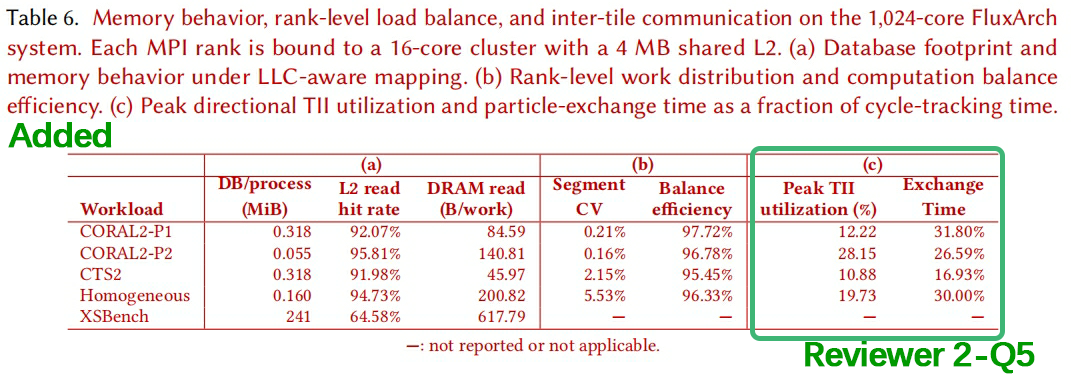
\includegraphics[width=0.9\textwidth]{news/R2-Q5-tab6c.png}}
\end{figure}
\end{minipage}\par\medskip

\item \textbf{Death-Respawn cost.} Death-Respawn and particle exchange are included in the evaluated execution path. We added an end-to-end timer covering send-buffer handling, MPI communication and waiting, receive-side particle management, and termination-related communication. This phase accounts for 16.93\%--31.80\% of cycle-tracking time, showing that it is material even though the modeled TIIs are not saturated.

\revisionlocation{The end-to-end particle-exchange measurement boundary and its distinction from pure link-transfer time are clarified in \textbf{Section 6.7}.}

\excerptlabel{Added (Section 6.7, page 21):}\par
\begin{manuscriptexcerpt}
\redsentence{Particle exchange nevertheless accounts for 16.93\%--31.80\% of cycle-tracking time.} \redsentence{This end-to-end phase includes send-buffer handling, MPI communication and waiting, receive-side particle management, and termination-related communication; it should therefore not be interpreted as pure link-transfer time.} \redsentence{Together, the measurements show that particle exchange has a measurable execution cost, but that cost cannot be attributed to saturation of the modeled TII bandwidth.}
\end{manuscriptexcerpt}
\par\noindent\begin{minipage}{\linewidth}
\revisionlocation{The particle-exchange share of cycle-tracking time is reported in \textbf{Table~6(c)}.}

\excerptlabel{Added (Table~6(c), page 18):}\par
% Revised manuscript: Table 6(c)
\begin{figure}[H]
  \centering
  \fbox{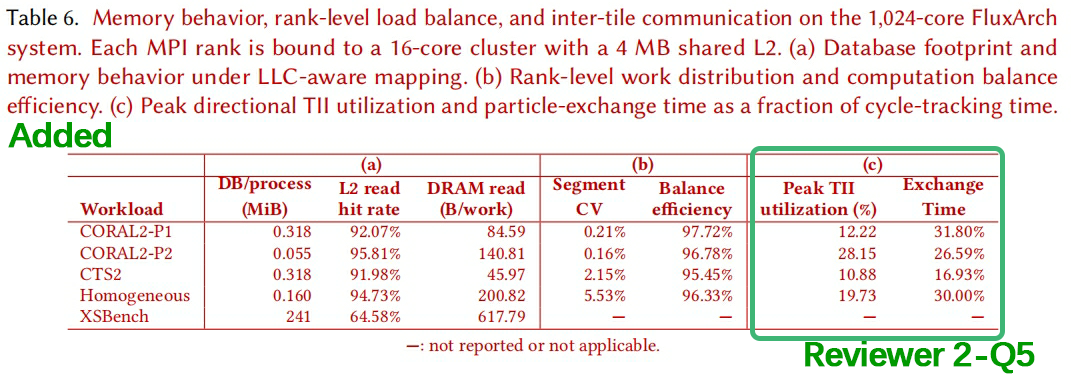
\includegraphics[width=0.9\textwidth]{news/R2-Q5-tab6c.png}}
\end{figure}
\end{minipage}\par\medskip

\item \textbf{MMIO programming and porting interface.} Each Engine is directly attached to its core's execute stage, as shown in \textbf{Figure~7}. Its MMIO interface addresses core-local registers, avoiding the interconnect traversal associated with remote MMIO peripherals. Ordinary loads and stores access the 64-bit register map, so the interface requires neither an ISA extension nor compiler modification. We clarified this local connection and added the complete operand order, launch sequence, completion protocol, and software-porting boundary in \textbf{Section 4.2} and added \textbf{Table~2(a)}. As described in \textbf{Section 6.4}, the evaluated execution path still includes the MMIO instructions, Engine synchronization, and Engine execution latency.

\revisionlocation{The core-local Engine connection, launch/completion protocol, and software-porting requirements are clarified in \textbf{Section 4.2}.}

\excerptlabel{Revised (Section 4.2, page 10):}\par
\begin{manuscriptexcerpt}
\redsentence{\textbf{Control and Programming Interface}.} \redsentence{As shown in Fig.~7, each \name\ Engine is directly attached to its core's execute stage.} \redsentence{Its memory-mapped interface provides software access to core-local registers, avoiding the interconnect traversal associated with remote MMIO peripherals.} \redsentence{The Control Unit maintains the iteration bounds and drives the nested loops in the FSM.} \redsentence{Through the 64-bit MMIO interface in Table~2(a), the host supplies the loop bounds; an accepted Control/Status write resets the internal counters and launches execution.} \redsentence{The host then streams operands and retrieves the results after \texttt{out\_valid} indicates completion.}

\redsentence{The interface is ISA-agnostic: the CPU performs database lookup in software, writes the resulting operands using ordinary stores, and reads the two final results using ordinary loads.} \redsentence{Porting therefore replaces only the stable software kernel with an MMIO wrapper; it requires neither ISA extensions nor changes to the compiler, particle representation, database layout, or MPI+OpenMP orchestration.}
\end{manuscriptexcerpt}

\par\noindent\begin{minipage}{\linewidth}
\revisionlocation{The operand order and software-visible register map are added in \textbf{Table~2(a)}.}

\excerptlabel{Added (Table~2(a), page 10):}\par
% Revised manuscript: Table 2(a)
\begin{figure}[H]
  \centering
  \fbox{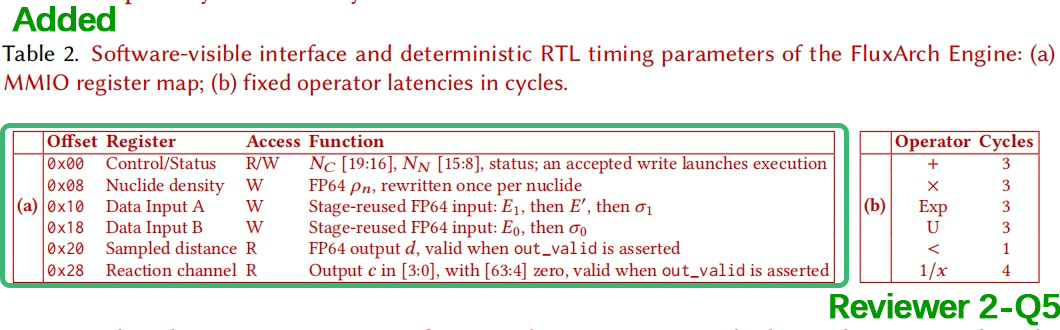
\includegraphics[width=0.9\textwidth]{news/R2-Q5-tab2a.png}}
\end{figure}
\end{minipage}\par\medskip

\item \textbf{Absolute throughput.} We supplemented normalized speedup with absolute throughput for every workload and platform. The revised results use segments/s for Quicksilver and lookups/s for XSBench and derive the normalized values from the same measurements. \name\ reaches 75.33--186.70 million segments/s across the Quicksilver inputs and 1.143 billion XSBench lookups/s.

\revisionlocation{The absolute throughput values and the units for Quicksilver and XSBench are specified in \textbf{Section 6.2}.}

\excerptlabel{Original (Section 6.2, page 14):}\par
\begin{manuscriptexcerpt}
\graysentence{\textbf{Performance Impact}.} \graysentence{Fig.~13(a) presents the performance of platforms across five benchmarks, normalized to the \ft.} \graysentence{The results underscore a cooperation between the domain-specific architecture and the synergistic workload orchestration.}

\graysentence{Without the synergistic workload orchestration, \name\ offers little to no advantage over CPUs and GPUs, ranging from 0.17$\times$ (vs. \hopper) to 1.54$\times$ (vs. \intel), due to severe interconnect contention and non-local memory traffic.} \graysentence{Crucially, enabling the workload orchestration unlocks the full potential of \name\ to surpass all of the platforms, boosting the geometric mean speedup from \textbf{1.02}$\boldsymbol{\times}$ (vs. \amd) to \textbf{6.83}$\boldsymbol{\times}$ (vs. \ft).}
\end{manuscriptexcerpt}

\excerptlabel{Revised (Section 6.2, page 15):}\par
\begin{manuscriptexcerpt}
\redsentence{\textbf{Performance Impact}.} \redsentence{Fig.~13(a,b) reports absolute throughput and values normalized to \ft.} \redsentence{\name\ achieves 79.33, 186.70, 75.33, and 123.50 million segments/s for P1, P2, CTS2, and Homo, respectively, and 1.143 billion XS lookups/s, yielding geometric-mean speedups from \textbf{1.02}$\boldsymbol{\times}$ over \amd\ to \textbf{6.83}$\boldsymbol{\times}$ over \ft.}
\end{manuscriptexcerpt}

\par\noindent\begin{minipage}{\linewidth}
\revisionlocation{The per-platform absolute throughput and corresponding normalized results are presented in \textbf{Figure~13(a,b)}. Panel (a) is newly added; panel (b) revises the original normalized-performance plot.}

\excerptlabel{Revised (Figure~13, page 16):}\par
% Revised manuscript: Figure 13
\begin{figure}[H]
  \centering
  \fbox{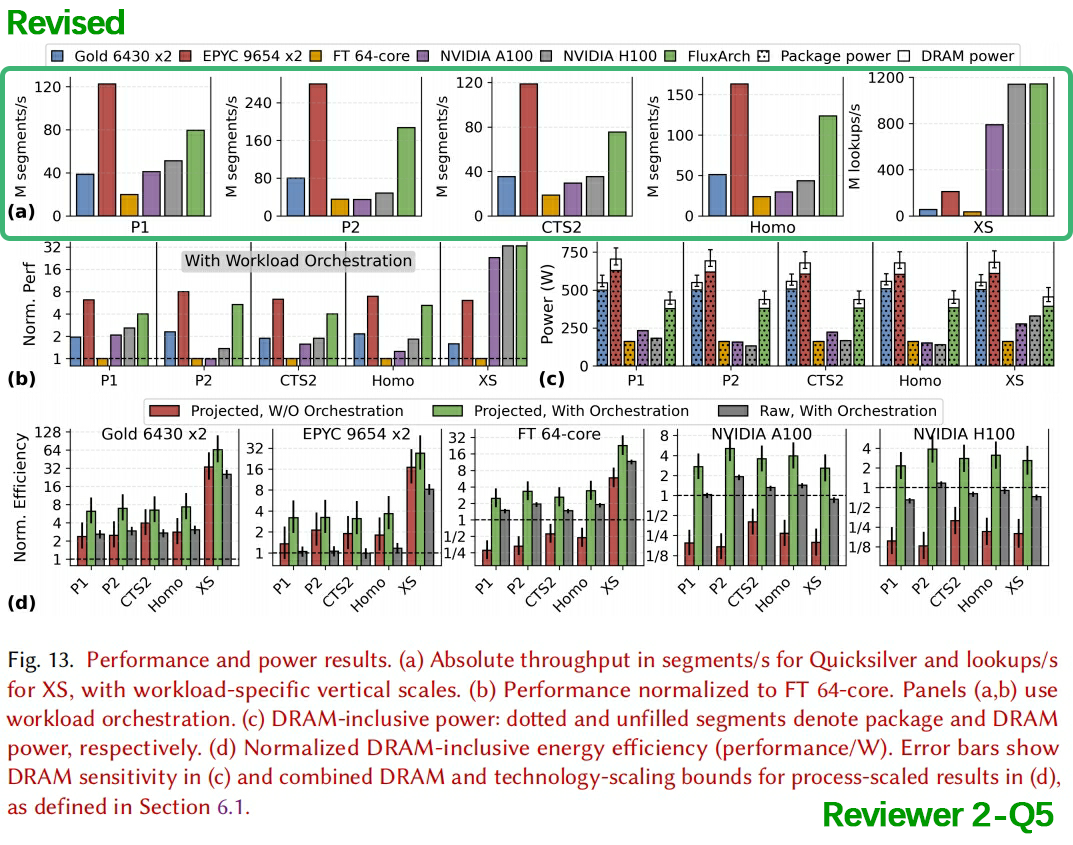
\includegraphics[width=0.9\textwidth]{news/R2-Q5-fig13a.png}}
\end{figure}
\end{minipage}\par\medskip

\item \textbf{Model validation against silicon.} As detailed in our response to \textbf{R2-Q1, item (2)}, six RK3562 silicon comparisons calibrate the core and cache/DRAM paths, with 6.7\% mean and 13.5\% maximum absolute percentage errors. The RTL-derived Engine timing establishes implementation traceability, not independent silicon validation; the complete 1,024-core hierarchy remains evaluated through calibrated simulation rather than a fabricated prototype. The supporting manuscript excerpts and calibration results are provided in that response. The distinction between native baseline measurements and simulated \name\ results is documented in \textbf{R2-Q1, item (1)}.\looseness=-1

\end{enumerate}

\clearpage
\section{Reviewer 3}

\subsection{Question 1}
\begin{reviewcomment}
The performance model is unvalidated. This is the central weakness.

FluxArch is evaluated in gem5, with McPAT and CACTI for power and area. The cores derive from real ARM in-order cores, which helps. The full system does not. A 1,024-core design with a custom dataflow engine, a tree interconnect, and a NUMA chiplet hierarchy is never checked against silicon, RTL, or an existing many-core platform. The only error bar in the paper (30\%) covers the technology-node power projection, not the timing model. Every performance and efficiency number depends on this uncalibrated model. The 6.83$\times$ speedup cannot be assessed without validation evidence.
\end{reviewcomment}
We sincerely thank you for your helpful and constructive suggestion. We agree that the performance claims require explicit validation evidence and a clear statement of what remains simulation-based. We therefore address the Engine, core/cache path, and complete system separately.

\begin{enumerate}[label=(\arabic*)]
\setlength{\emergencystretch}{1em}
\item \textbf{RTL-derived Engine timing.} The Engine is a deterministic dataflow implementation whose latency depends on the nuclide count ($N_N$) and reaction-channel count per nuclide ($N_C$) rather than on operand values. We added an RTL-to-gem5 derivation using the fixed operator latencies and the dependencies among the five stages. This produces the closed-form computation latency $12N_NN_C+10N_N+4N_C+3$, which gem5 implements directly instead of fitting an empirical delay.

\revisionlocation{The deterministic Engine timing expression and its RTL derivation are explained in \textbf{Section 4.2}.}

\par\noindent\begin{minipage}{\linewidth}
\excerptlabel{Figure~9 (page 9):}\par
% Manuscript: Figure 9
\begin{figure}[H]
  \centering
  \fbox{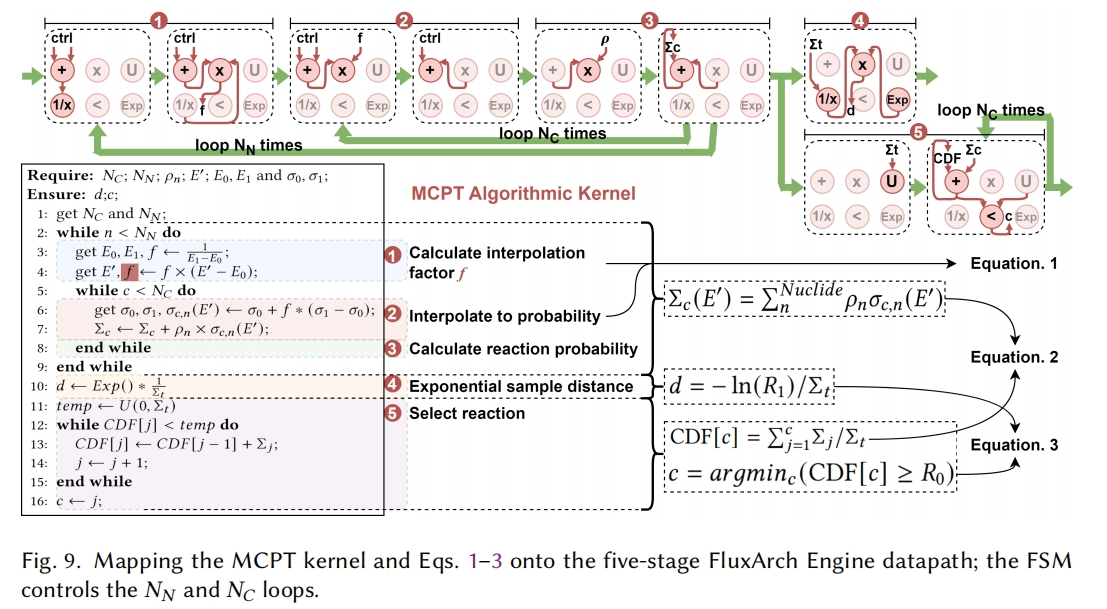
\includegraphics[width=0.9\textwidth]{figures/fig9.png}}
\end{figure}
\end{minipage}\par\medskip

\excerptlabel{Added (Section 4.2, pages 9--10):}\par
\begin{manuscriptexcerpt}
\redsentence{Here, $N_N$ denotes the number of nuclides and $N_C$ the number of reaction channels per nuclide; they determine the outer and inner loop bounds, respectively.}

\redsentence{\textbf{Deterministic Timing Model.}} \redsentence{To meet the timing requirements at the same target clock frequency as the \name\ Core, the RTL operators are partitioned into different numbers of pipeline stages.} \redsentence{Table~2(b) lists the fixed RTL operator latencies using the same symbols as Fig.~9.} \redsentence{Under the computation-only boundary used by the Engine model---excluding launch, stage-transition, \texttt{out\_valid}, and CPU/MMIO input-wait cycles---the five stages take 10 cycles for \redone~($+\to1/x\to\times$, $3+4+3$), 12 cycles for \redtwo~and \redthree~combined~($+\to\times\to+\to\times$, $3+3+3+3$), 7 cycles for \redfour~($1/x\to\times$, $4+3$), and $3+4N_C$ cycles for \redfive~($U\to\{+\to<\}^{N_C}$, $3+N_C(3+1)$).} \redsentence{The resulting latency is
\[
\begin{array}{rl}
L_{\mathrm{Engine}}(N_N,N_C)
&=N_N(10+12N_C)+\max(7,3+4N_C) \\
&=12N_NN_C+10N_N+4N_C+3.
\end{array}
\]} \redsentence{It depends only on the programmed nuclide and reaction-channel counts, not on the numerical operand values.} \redsentence{The gem5 Engine timing directly implements this RTL-derived expression rather than an empirically fitted latency.}
\end{manuscriptexcerpt}

\par\noindent\begin{minipage}{\linewidth}
\revisionlocation{The operator latencies and five-stage timing parameters are specified in \textbf{Table~2(b)}.}

\excerptlabel{Added (Table~2, page 10):}\par
% Revised manuscript: Table 2
\begin{figure}[H]
  \centering
  \fbox{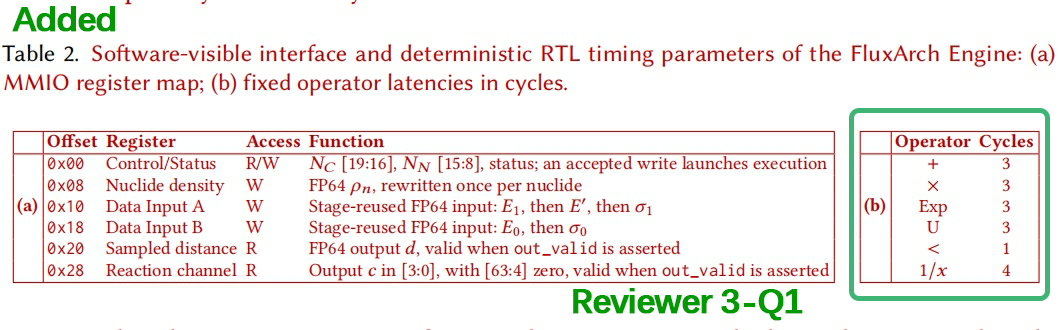
\includegraphics[width=0.9\textwidth]{news/R3-Q1-tab2b.png}}
\end{figure}
\end{minipage}\par\medskip

\item \textbf{Silicon-based core and memory calibration.} The in-order core and cache/DRAM paths are anchored to a Cortex-A53-class silicon reference. We now report the details of six matched native/simulated configurations spanning integer execution, branch control, and dependent random accesses from 16 KiB to 64 MiB. All checksums match, while the measured latency differences yield 6.7\% mean absolute percentage error and 13.5\% maximum absolute percentage error.

\revisionlocation{The silicon-based core and memory calibration protocol, accuracy, and scope are described in \textbf{Section 6.1}.}

\excerptlabel{Added (Section 6.1, page 13):}\par
\begin{manuscriptexcerpt}
\redsentence{\textbf{Core Timing Calibration}.} \redsentence{We calibrate the 2-GHz in-order \name\ Core model against a 2-GB KickPi K3B with a 22-nm quad-core RK3562 Cortex-A53~\papercite{kickpi-k3b,rockchip-rk3562}.} \redsentence{The native process is pinned to one 2-GHz core under stable thermal conditions; both platforms use identical source, GCC 13.3, \texttt{-O2 -fno-tree-vectorize}, seed, warm-up, and timed region.} \redsentence{All six checksums match.} \redsentence{Table~3 reports latency and signed error $100(T_{\rm gem5}-T_{\rm K3B})/T_{\rm K3B}$; across the six tests, the mean and maximum absolute percentage errors are 6.7\% and 13.5\%, respectively.} \redsentence{FluxArch's absolute throughput and speedups are obtained directly from the calibrated simulations.}
\end{manuscriptexcerpt}
\begin{excerptreferences}
\paperreference{rockchip-rk3562}
\paperreference{kickpi-k3b}
\end{excerptreferences}
\par\noindent\begin{minipage}{\linewidth}
\revisionlocation{The six matched RK3562 calibration cases and their latency errors are reported in \textbf{Table~3}.}

\excerptlabel{Added (Table~3, page 13):}\par
% Revised manuscript: Table 3
\begin{figure}[H]
  \centering
  \fbox{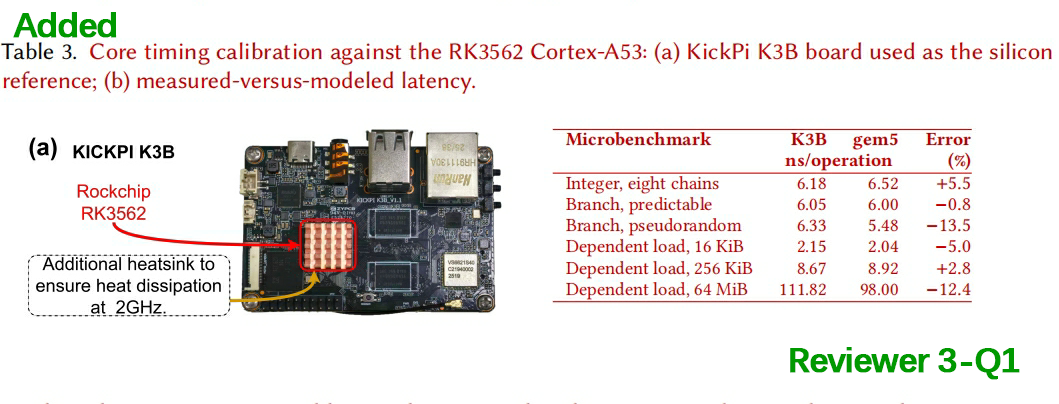
\includegraphics[width=0.9\textwidth]{news/R3-Q1-tab3.png}}
\end{figure}
\end{minipage}\par\medskip



\item \textbf{Performance with the calibrated model.} The performance results reported in \textbf{Section~\ref{subsec:performance_and_power}} and \textbf{Fig.~\ref{fig:perfandpower}(a,b)} already use the calibrated model described above; this revision makes the calibration and RTL timing details explicit. The table below summarizes \name's speedup relative to each evaluated platform with workload orchestration. Each entry is the ratio of \name\ throughput to the platform throughput for the same workload; the final column is the geometric mean of the five ratios.

\par\medskip\noindent\begin{minipage}{\linewidth}
\centering
\small
\textbf{\name\ speedup relative to each platform ($\times$).}\par\smallskip
\setlength{\tabcolsep}{2.5pt}
\begin{tabular}{lrrrrrr}
\hline
\textbf{Platform} & \textbf{CORAL2-P1} & \textbf{CORAL2-P2} & \textbf{CTS2} & \textbf{Homogeneous} & \textbf{XSBench} & \textbf{Geo. mean} \\
\hline
\intel  & 2.05 & 2.33 & 2.13 & 2.42 & 20.98 & \textbf{3.49} \\
\amd    & 0.65 & 0.67 & 0.63 & 0.76 & 5.44 & \textbf{1.02} \\
\ft     & 4.00 & 5.34 & 4.02 & 5.22 & 33.20 & \textbf{6.83} \\
\ampare & 1.93 & 5.38 & 2.57 & 4.16 & 1.45 & \textbf{2.76} \\
\hopper & 1.55 & 3.89 & 2.14 & 2.85 & 1.00 & \textbf{2.06} \\
\hline
\end{tabular}
\end{minipage}\par\medskip

In particular, the 6.83$\times$ figure is the five-workload geometric-mean speedup over FT 64-core, not a uniform speedup across workloads or platforms. These results are supported by silicon-based core/memory calibration and RTL-derived Engine timing.

\end{enumerate}

\subsection{Question 2}
\begin{reviewcomment}
The energy claim excludes DRAM, and the effect is not bounded.

The paper reports large energy-efficiency gains but excludes off-chip DRAM power. MCPT is memory-bound. The paper's own data (Fig. 3(d)(e)) shows the working set exceeds on-chip capacity and forces frequent DRAM access. DRAM energy is therefore likely a large share of system energy. The on-chip scope is disclosed, which is fair. The problem is that the impact is never quantified. A system-level energy result could be materially smaller. As written, the energy advantage is an architectural-efficiency claim, not a system claim, and the gap between the two is unknown.
\end{reviewcomment}
We agree that the original on-chip-only comparison could not support a system-level energy claim for a memory-bound workload. We changed the evaluation to include co-packaged memory through platform telemetry and off-package DDR5 through a common traffic-based DRAMPower model, and we vary the modeled DDR5 component over a $0.5\times$--$2\times$ range to assess sensitivity to missing command-level detail. The conservative process-scaled geometric-mean DRAM-inclusive energy-efficiency advantage remains 1.77$\times$ over H100 and 6.65$\times$ over Intel.

We now explain the choice of the $0.5\times$--$2\times$ range in \textbf{Section 6.1}. Ghose et al.~\papercite{ghose2018vampire} measured DDR3L read currents averaging 54.1\% below datasheet values for one vendor and data-pattern-dependent read-power differences of up to 91.6\%. Shi et al.~\papercite{shi2025drampower} report that DDR4 calibration reduced DRAMPower energy estimates by roughly half for most evaluated SPEC2006 workloads. These results motivate testing sizable modeling discrepancies, but do not establish an error bound for our DDR5 configuration. We therefore select reciprocal factors of 0.5 and 2 to test both overestimation and underestimation, with package power fixed; the range is a sensitivity-analysis choice, not a statistical confidence interval.

For process-scaled energy-efficiency bounds, we independently vary only the scaled FluxArch package power by $\pm30\%$ and each modeled off-package DRAM component over $0.5\times$--$2\times$, while keeping throughput and measured baseline package power fixed. We recompute the performance/W ratio at every endpoint combination and report its minimum and maximum; external DRAM power is not subject to process-node scaling or its 30\% margin.


\revisionlocation{The power-accounting boundary is revised in \textbf{Section 6.1} to include DRAM consistently across platforms.}

\excerptlabel{Revised (Section 6.1, page 14):}\par
\begin{manuscriptexcerpt}
\redsentence{We report DRAM-inclusive system power and energy.} \redsentence{Package power includes cores, caches, NoCs, and integrated memory controllers; for \ft, \ampare, and \hopper, the main memory is co-packaged (DDR4 or HBM) and is consequently covered by platform-level package/device telemetry.} \redsentence{In contrast, the DDR5 DIMMs of \intel\ and \amd, and the DDR5 channels assumed for \name, are physically off-package and are not covered by package-power readings.} \redsentence{We therefore add a separately modeled DRAM component to these platforms, avoiding asymmetric accounting that would include HBM/DDR4 power for the co-packaged-memory platforms but omit DDR5 power for the other platforms.}

\end{manuscriptexcerpt}

\revisionlocation{The traffic-based DRAM model and factor-of-two sensitivity analysis are added in \textbf{Section 6.1}.}

\excerptlabel{Added (Section 6.1, pages 14--15):}\par
\begin{manuscriptexcerpt}
\redsentence{For the DRAM model, we use DRAMPower 5~\papercite{drampower} with DDR5 timing and worst-case current parameters from the JEDEC DDR5 standard~\papercite{jedec_ddr5} and the Micron MT60B2G8HB-48B DDR5-4800 x8 datasheet~\papercite{micron_ddr5}.} \redsentence{\name\ is modeled with 32 single-rank DDR5-4800 channels, each containing eight x8 DRAM devices.} \redsentence{The model includes active-standby background power, refresh power, and read/write transfer power.} \redsentence{The external-memory energy of \intel\ and \amd\ is estimated using the same traffic-based DDR5 model and workload-specific memory traffic.}

\redsentence{Because the simulation does not expose DRAM command traces or row-buffer events, we use a traffic-based DRAM energy estimate rather than claiming command-level precision.} \redsentence{For each \name\ workload, we derive read/write traffic from the memory-system statistics and use the simulated execution time.} \redsentence{Prior DRAM measurement and calibration studies report substantial discrepancies between datasheet-based estimates and measured consumption~\papercite{ghose2018vampire,shi2025drampower}.} \redsentence{Motivated by these findings, we select a $0.5\times$--$2\times$ range for the nominal modeled DRAM power of every off-package DDR5 platform (\intel, \amd, and \name).} \redsentence{This range is a sensitivity-analysis choice, not an empirically established DDR5 error bound or a statistical confidence interval.}
\end{manuscriptexcerpt}
\begin{excerptreferences}
\paperreference{drampower}
\paperreference{jedec_ddr5}
\paperreference{micron_ddr5}
\paperreference{ghose2018vampire}
\paperreference{shi2025drampower}
\end{excerptreferences}

\revisionlocation{The energy-efficiency comparison and conservative lower bounds are updated in \textbf{Section 6.2} to include DRAM power.}

\excerptlabel{Original (Section 6.2, pages 14--15):}\par
\begin{manuscriptexcerpt}
\graysentence{\textbf{Iso-Process Energy Efficiency}.} \graysentence{As shown in Fig.~13(b), the energy efficiency advantage is even more pronounced.} \graysentence{By comparing projected iso-process nodes, we isolate the architectural contributions.} \graysentence{According to Section 6.1, the power projection error is 30\%.} \graysentence{Therefore, we incorporate this margin into our energy efficiency evaluation, which is represented as error bars in our results.}

\graysentence{Without the workload orchestration, the energy efficiency of \name, mainstream server CPUs and high-end GPUs is at odds with each other.} \graysentence{With the orchestration enabled, optimizing data locality and minimizing cross-tile traffic, \name\ demonstrates a superior geometric mean energy efficiency improvement from \textbf{3.98}$\boldsymbol{\times}$ (vs. \ft, 5.69$\times$ discounted by 30\%) to \textbf{9.84}$\boldsymbol{\times}$ (vs. \intel, 14.06$\times$ discounted by 30\%) even accounting for the potential projection error of pessimistic assumption.} \graysentence{We also report the energy efficiency of the raw, unscaled data based on the 22 nm technology node.} \graysentence{Even in this case, \name\ still achieves an energy efficiency improvement of 1.17$\times$ (vs. \hopper) to 4.59$\times$ (vs. \intel).}
\end{manuscriptexcerpt}

\excerptlabel{Revised (Section 6.2, pages 15--16):}\par
\begin{manuscriptexcerpt}
\redsentence{\textbf{DRAM-Inclusive Energy Efficiency}.} \redsentence{Fig.~13(c,d) reports DRAM-inclusive power and energy efficiency under the sensitivity bounds defined in Section~6.1.} \redsentence{Process-scaled results separate architectural effects from process scaling while accounting consistently for external memory.}

\redsentence{In the process-scaled comparison, \name\ improves geometric-mean DRAM-inclusive efficiency by \textbf{2.85}$\boldsymbol{\times}$ over \hopper\ to \textbf{10.58}$\boldsymbol{\times}$ over \intel.}

\redsentence{The sensitivity analysis preserves the process-scaled conclusion: across the combined DRAM and technology-scaling bounds, the geometric-mean improvement with orchestration remains 1.77$\times$ over \hopper\ and 6.65$\times$ over \intel\ at the conservative lower bound.}
\end{manuscriptexcerpt}

\revisionlocation{The energy-efficiency claim is updated in \textbf{Section 9} to reflect the process-scaled, DRAM-inclusive results.}

\excerptlabel{Original (Section 9, page 20):}\par
\begin{manuscriptexcerpt}
\graysentence{We introduced \name, a thousand-core architecture that addresses the performance bottlenecks of MCPT through a large-scale MIMD design and specialized dataflow engines.} \graysentence{By co-optimizing hardware topology and spatial decomposition, \name\ overcomes irregular memory access limitations and delivers geometric mean speedups of up to 1.02$\times$--6.83$\times$ and energy efficiency improvements of up to 3.98$\times$--9.84$\times$ over traditional processors.}
\end{manuscriptexcerpt}

\excerptlabel{Revised (Section 9, page 23):}\par
\begin{manuscriptexcerpt}
\graysentence{We introduced \name, a thousand-core architecture that addresses the performance bottlenecks of MCPT through a large-scale MIMD design and specialized dataflow engines.} \redsentence{It also delivers process-scaled DRAM-inclusive energy-efficiency improvements of 2.85$\times$--10.58$\times$.}
\end{manuscriptexcerpt}

\par\noindent\begin{minipage}{\linewidth}
\revisionlocation{The DRAM-inclusive power and energy-efficiency plots are updated in \textbf{Figure~13(c,d)}. Panel (c) is newly added; panel (d) revises the original energy-efficiency plot.}

\excerptlabel{Revised (Figure~13, page 16):}\par
% Revised manuscript: Figure 13
\begin{figure}[H]
  \centering
  \fbox{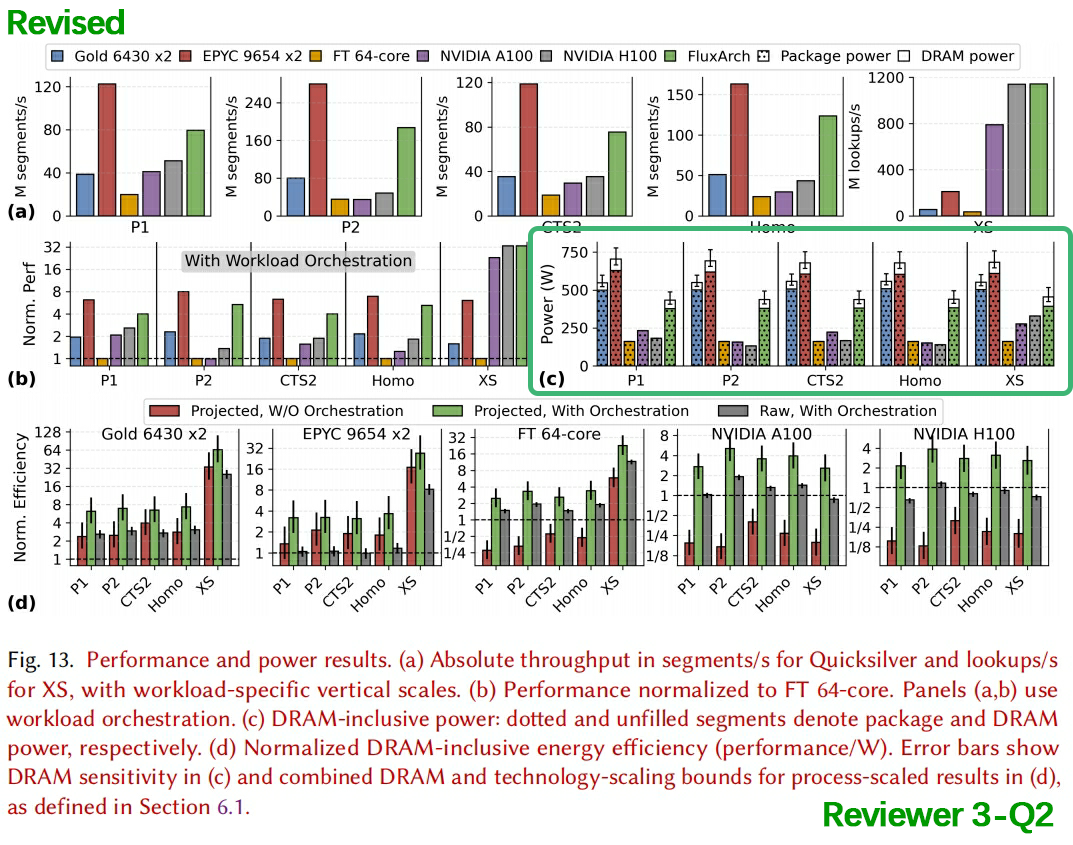
\includegraphics[width=0.9\textwidth]{news/R3-Q2-fig13.png}}
\end{figure}
\end{minipage}\par\medskip

\subsection{Question 3}
\begin{reviewcomment}
The baseline comparison has two specific gaps.

One benchmark (EMCP) is an event-based proxy, and the orchestration is applied to the CPU baselines, so the baselines are not naive. Two gaps remain. Particle-sorting MCPT methods are not evaluated, despite being a known GPU optimization. The comparison against prior specialized MCPT architectures is qualitative only (Table 4); there is no quantitative speedup against those designs. Without these, the claim of superiority over the state of the art is incomplete.
\end{reviewcomment}
We sincerely thank you for your helpful and constructive suggestion. We address the two baseline gaps separately.

\begin{enumerate}[label=(\arabic*)]
\setlength{\emergencystretch}{1em}
\item \textbf{Particle-sorting GPU baseline.} The GPU baseline now includes the particle-sorting optimization rather than comparing only against an unsorted implementation. We evaluated XSBench CUDA variants K4--K6 on both A100 and H100 with sampling, sorting, lookup, and reduction included in the timed and power-measurement interval, and selected the best end-to-end variant, K6. The strengthened H100 baseline reaches 1.140 billion lookups/s, nearly matching \name's 1.143 billion lookups/s; the five-workload geometric-mean speedup of \name\ over H100 is consequently 2.06$\times$.


\revisionlocation{The sorting-enabled GPU baseline selection and end-to-end timing/power boundary are specified in \textbf{Section 6.1}.}

\excerptlabel{Added (Section 6.1, page 14):}\par
\begin{manuscriptexcerpt}
\redsentence{\textbf{GPU Particle-Sorting Baseline}.} \redsentence{For the GPU XSBench baseline, we evaluate the sorting-enabled CUDA variants K4--K6, which group cross-section lookups by material, fuel category, and/or particle energy to reduce warp divergence and improve memory locality.} \redsentence{We use the variant with the highest end-to-end throughput on each GPU; K6, which combines material and energy sorting with material-specific kernels, is the best-performing evaluated variant on both \ampare\ and \hopper.} \redsentence{The reported runtime includes sampling, sorting, cross-section lookup, and result reduction, and the corresponding GPU-board power covers the same execution interval.}
\end{manuscriptexcerpt}

\revisionlocation{The K6 throughput and the resulting comparison with FluxArch are updated in \textbf{Section 6.2}.}

\excerptlabel{Added (Section 6.2, page 15):}\par
\begin{manuscriptexcerpt}
\redsentence{The selected K6 baseline reaches 788.63 million and 1.140 billion XS lookups/s on \ampare\ and \hopper, respectively.} \redsentence{Thus, \name\ and \hopper\ provide nearly identical XS throughput (1.143 versus 1.140 billion lookups/s), while \name's five-workload geometric-mean advantage over \hopper\ is 2.06$\times$.}
\end{manuscriptexcerpt}

\par\noindent\begin{minipage}{\linewidth}
\revisionlocation{The absolute throughput and normalized-performance plots are updated in \textbf{Figure~13(a,b)} using the sorting-enabled GPU baseline. Panel (a) is newly added; panel (b) revises the original normalized-performance plot.}

\excerptlabel{Revised (Figure~13, page 16):}\par
% Revised manuscript: Figure 13
\begin{figure}[H]
  \centering
  \fbox{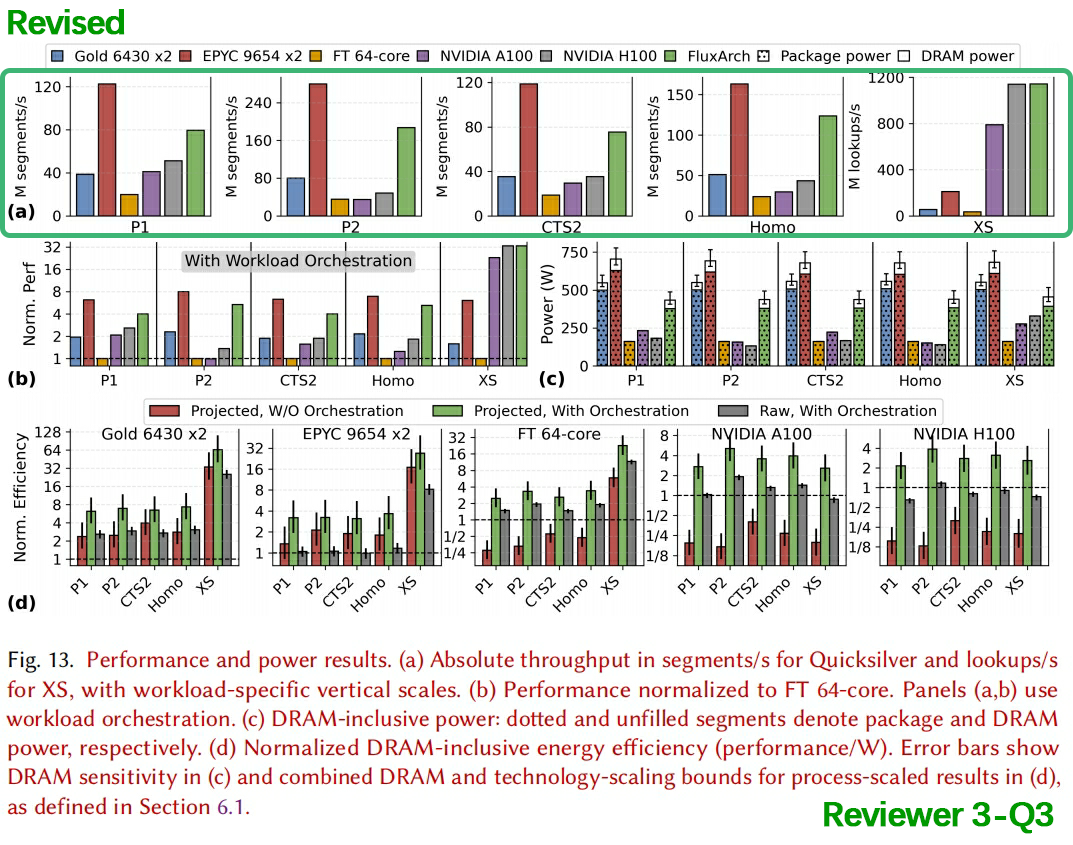
\includegraphics[width=0.9\textwidth]{news/R3-Q3-fig13.png}}
\end{figure}
\end{minipage}\par\medskip

\item \textbf{Prior specialized MCPT architectures.} We added \textbf{Table~7} to compare \name\ with the closely related designs of Fu et al. and Zhang et al., including their core design, hierarchy, cache and memory organization, methodology, workloads, and author-reported quantitative results.

As clarified in \textbf{Section 8}, these results use different workload inputs, resources, baselines, and accounting boundaries. Fu et al.'s ratios are relative to a four-core Cortex-A15 model, whereas Zhang et al.'s scaling efficiency is relative to their own single-core configuration. They therefore cannot be converted into direct speedups over these designs.

A common reimplementation would also require assumptions about implementation and modeling choices not fully specified in the papers. In particular, Zhang et al. do not report a process node or a power/area model. Reconstructing customized simulator configurations and adding such models could make the comparison depend on reconstruction choices as well as architectural differences. We added this limitation to \textbf{Section 8}, rather than presenting assumption-dependent estimates as a validated head-to-head comparison.

\revisionlocation{The comparison with Fu et al. and Zhang et al. is revised in \textbf{Section 8} to clarify the architectural differences.}

\excerptlabel{Original (Section 8, page 19):}\par
\begin{manuscriptexcerpt}
\graysentence{Recent microarchitectural studies have shifted toward specialized, area-efficient designs.} \graysentence{Fu et al. pioneered the use of clustered small cores to improve energy-to-area ratios for MCPT workloads, a foundation subsequently extended by Zhang et al. to a 128-core cluster with optimized parallelization.} \graysentence{Our \name\ system achieves a significant leap forward by: (1) scaling the architecture to 1,024 cores using a hierarchical chiplet-based design; (2) integrating a dedicated execution engine to offload dominant kernels; and (3) proposing a topology-aware hardware-software co-design that transcends the scalability limits of prior clustered small-core architectures.}
\end{manuscriptexcerpt}

\excerptlabel{Revised (Section 8, page 22):}\par
\begin{manuscriptexcerpt}
\redsentence{\textbf{Specialized MCPT Architectures.}} \graysentence{Recent microarchitectural studies have shifted toward specialized, area-efficient designs.} \redsentence{Table~7 compares \name\ with Fu et al.~\papercite{minimctad} and Zhang et al.~\papercite{128mc} in core design, hierarchy, cache and memory organization, evaluation methodology, workloads, and author-reported results.} \redsentence{Fu et al. use simplified in-order cores to improve area and power efficiency, while Zhang et al. scale to 128 cores through 32-core cache-sharing clusters and OpenMP dynamic scheduling.} \redsentence{\name\ combines a 1,024-core hierarchy with a core-local Engine and topology-aware spatial mapping.}

\end{manuscriptexcerpt}
\begin{excerptreferences}
\paperreference{minimctad}
\paperreference{128mc}
\end{excerptreferences}

\revisionlocation{The limits of comparing published results and reconstructing prior designs fairly are added in \textbf{Section 8}.}

\excerptlabel{Added (Section 8, page 22):}\par
\begin{manuscriptexcerpt}
\redsentence{The reported results use substantially different experimental conditions, including workload inputs, core counts, cache and memory configurations, reference baselines, and power-accounting boundaries.} \redsentence{Fu et al. report performance, performance/W, and performance/area relative to a modeled four-core Cortex-A15 system.} \redsentence{Zhang et al. report scaling efficiency relative to their own single-core configuration.} \redsentence{\name's performance and energy-efficiency ratios use the evaluated CPU/GPU platforms as baselines, whereas its scaling efficiency is relative to one core.} \redsentence{Thus, Table~7 places each work's results in context rather than establishing cross-architecture speedups or an efficiency ranking.}

\redsentence{A unified reimplementation would also require resolving implementation and modeling choices not fully specified in the papers, rather than merely matching their listed hardware parameters.} \redsentence{In particular, Zhang et al. do not report a process node or a power/area model.} \redsentence{Reconstructing the customized simulator configurations and supplying missing power/area models would introduce additional assumptions that could affect the results, confounding architectural differences with reconstruction choices and weakening the fairness of a direct comparison.}


\end{manuscriptexcerpt}


\par\noindent\begin{minipage}{\linewidth}
\revisionlocation{The detailed architectural comparison and author-reported quantitative results are added in \textbf{Table~7}.}

\excerptlabel{Added (Table~7, page 22):}\par
% Revised manuscript: Table 7
\begin{figure}[H]
  \centering
  \fbox{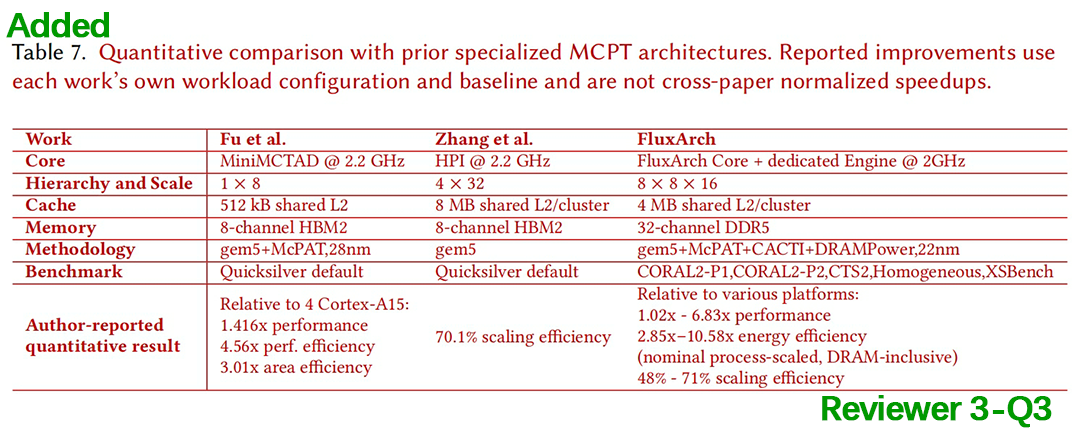
\includegraphics[width=0.9\textwidth]{news/R3-Q3-tab7.png}}
\end{figure}
\end{minipage}\par\medskip

\end{enumerate}


\end{document}
